
\documentclass{article}


\usepackage[margin=1in]{geometry}
\usepackage{hyperref}
\usepackage{comment}
\usepackage{graphicx}
\usepackage{tabularx}
\usepackage{array}
\usepackage{xcolor}
\usepackage{tcolorbox}
\usepackage{float}
\usepackage{caption}

\newcolumntype{L}{>{\arraybackslash}p{14cm}}
\newcolumntype{C}{>{\centering\arraybackslash}p{1.8cm}}
\newcommand{\centered}[1]{\begin{tabular}{l} #1 \end{tabular}}
\newcommand{\centeredl}[1]{\begin{tabular}{p{14cm}} #1 \end{tabular}}

\newtcolorbox{code}{colback=blue!10,colframe=white}
\newtcolorbox{msg}{colback=yellow!10,colframe=white}
\newtcolorbox{goal}{colback=green!10,colframe=white}

\colorlet{darkpink}{red!60}
\colorlet{darkred}{red!60!black!100}
\colorlet{lightpurple}{purple!70!blue!70}
\colorlet{darkblue}{blue!60!black!100}
\colorlet{darkgreen}{green!40!black!100}
\colorlet{teal}{green!50!blue!100}

\newcommand{\blue}[1]{\textcolor{blue}{#1}}

\newcommand{\cmd}[1]{\textcolor{lightpurple}{#1}}
\newcommand{\cmt}[1]{\textcolor{darkred}{(* #1 *)}}
\newcommand{\str}[1]{\textcolor{darkpink}{#1}}

\newcommand{\nm}[1]{\textcolor{darkblue}{#1}}
\newcommand{\df}[1]{\textcolor{red}{#1}}
\newcommand{\ty}[1]{\textcolor{teal}{#1}}
\newcommand{\kw}[1]{\textcolor{darkgreen}{#1}}


\newcommand{\Type}{\ty{Type}\ }
\newcommand{\Set}{\ty{Set}\ }

\newcommand{\Inductive}{\df{Inductive}\ }
\newcommand{\Definition}{\df{Definition}\ }
\newcommand{\Fixpoint}{\df{Fixpoint}\ }

\newcommand{\Theorem}{\df{Theorem}\ }
\newcommand{\Lemma}{\df{Lemma}\ }
\newcommand{\Example}{\df{Example}\ }

\newcommand{\Proof}{\cmd{Proof}}
\newcommand{\Qed}{\cmd{Qed}}
\newcommand{\Admitted}{\cmd{Admitted}}
\newcommand{\Abort}{\cmd{Abort}}

\newcommand{\Load}{\cmd{Load}\ }
\newcommand{\Check}{\cmd{Check}\ }
\newcommand{\Notation}{\cmd{Notation}\ }

\newcommand{\match}{\kw{match}\ }
\newcommand{\with}{\kw{with}\ }
\newcommand{\End}{\kw{end}}
\newcommand{\If}{\kw{if}\ }
\newcommand{\Then}{\kw{then}\ }
\newcommand{\Else}{\kw{else}\ }
\newcommand{\Forall}{\kw{forall}\ }
\newcommand{\as}{\kw{as}\ }
%\newcommand{\}{\{}\ }

\newcommand{\iconsize}{1.25cm}
\newcommand{\halfsize}{8cm}





\title{\textbf{The Coq Proof Assistant Tutorial} 
	\\ Software Verification}
\author{Amy Pritchard 
	\\ University at Buffalo, SUNY
	\\ amypritc@buffalo.edu}
\date{Last Update: Winter 2019}

\begin{document}
\maketitle

\begin{center}
	CoqIDE v8.10.2 (Updated up to Section \ref{bool_expr})
\\~\\
	CoqIDE v8.7.2 (to be removed once fully updated)
\end{center}

\vfill
\noindent
{\footnotesize Note: Screenshots and tutorial are based on the CoqIDE for MacOS - there may be differences between OS versions. }

\newpage
\tableofcontents


\newpage
\part{Introduction}
	\label{Part: intro}
\section{The COQ Proof Assistant Web Page} 
	\label{Sec: webpage}
	{\bf \url{https://coq.inria.fr}}

~\\
Here you can find all sorts of info about the COQ Proof Assistant, including the following: 

\begin{itemize}
\item About COQ (\url{https://coq.inria.fr/about-coq})

\item Getting COQ (\url{https://coq.inria.fr/download})

\item Documentation, i.e. books, tutorials, etc. (\url{https://coq.inria.fr/documentation})

\item Reference Manual (\url{https://coq.inria.fr/distrib/current/refman/}). 

\item Standard Library (\url{https://coq.inria.fr/distrib/current/stdlib/})

\item Community for discussion, contribution, events, etc. (\url{https://coq.inria.fr/community})

\item News about new releases (\url{https://coq.inria.fr/news/})

\end{itemize}














~\\~\\~\\
\section{Installation} 
	\label{Sec: installation}
	
For general installation options and instructions, go to
\url{https://coq.inria.fr/download}.

~\\
To get an installer for Windows or MacOS, go to 
\url{https://github.com/coq/coq/releases/latest}
and scroll down to the bottom of the page.

~\\
To install Coq via OPAM on MacOS or Linux, go to 
\url{https://coq.inria.fr/opam-using.html}
for step by step instructions.
 


\newpage
\section{The Coq IDE} 
	\label{Sec: ide}
	



\subsection{CoqIDE version 8.10.2}
	


\begin{minipage}{\linewidth}
\center{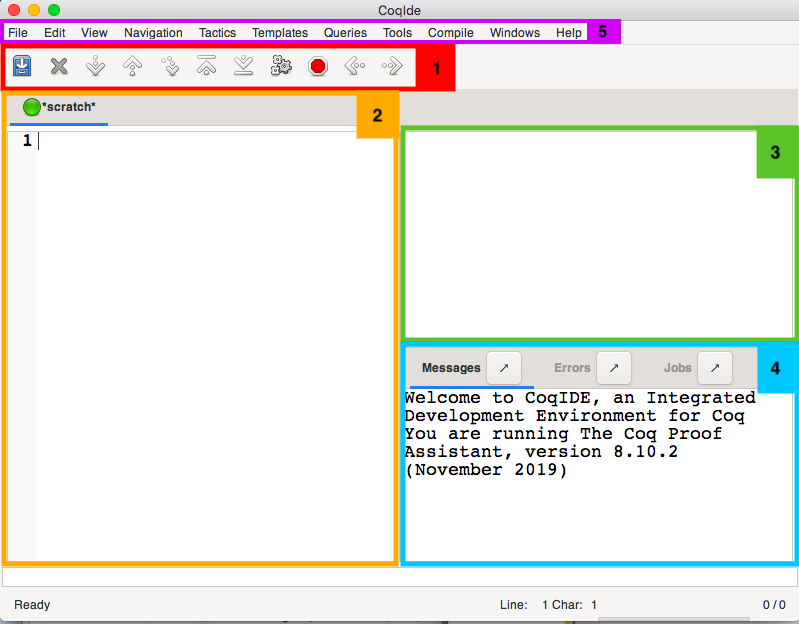
\includegraphics[width=\textwidth]
        {CoqScreenshots/CoqIDEv8_10_2_color.png}}
        \label{fig:IDEcolor} 
        \captionof{figure}{CoqIDE v8.10.2  
        (1) Toolbar. (2) Script Buffer. (3) Goal Window. (4) Message Window. }
\end{minipage}

\subsubsection{Toolbar for CoqIDE v8.10.2}
\hspace{-0.75cm}
\begin{tabular}{ C L }
\centered{
\includegraphics[width=\iconsize]
        {CoqScreenshots/save_10.png}}
        & \centeredl{Save current buffer. 
        If it hasn't been previously saved, functions as save as; use the extension .v to save as a Coq file.
        } \\ \\
\centered{
\includegraphics[width=\iconsize]
        {CoqScreenshots/close_10.png}}
	& \centeredl{Close current buffer. 
	Gives a warning if the file has unsaved changes.
	} \\ \\
\centered{
\includegraphics[width=\iconsize]
        {CoqScreenshots/step_forward_10.png}}
	& \centeredl{Forward one command.
	Steps forward to evaluate the next command in the current file.
	} \\ \\
\centered{
\includegraphics[width=\iconsize]
        {CoqScreenshots/step_backward_10.png}}
	& \centeredl{Backward one command.
	Steps backward one command in the file, returns the state to where it was before evaluating that command. 
	} \\ \\ 
\centered{
\includegraphics[width=\iconsize]
        {CoqScreenshots/go_to_cursor_10.png}}
	& \centeredl{Go to cursor.
	Evaluate all commands in file up to where the cursor currently is.
	} \\ \\ 
\centered{
\includegraphics[width=\iconsize]
        {CoqScreenshots/go_to_top_10.png}}
	& \centeredl{Restart Coq.
	Returns to the top of the file, where no commands have been evaluated.
	} \\ \\ 
\centered{
\includegraphics[width=\iconsize]
        {CoqScreenshots/go_to_bottom_10.png}}
	& \centeredl{Go to end.
	Evaluate to the bottom of the file. 
	Does not work as well with load commands and require import commands.
	} \\ \\
\centered{
\includegraphics[width=\iconsize]
        {CoqScreenshots/check_10.png}}
	& \centeredl{Fully check the document.
	Submits proof terms to the Coq kernel for type checking.
	} \\ \\
\centered{
\includegraphics[width=\iconsize]
        {CoqScreenshots/stop_10.png}}
	& \centeredl{Interrupt computations.
	Stops computation at whatever point was reached before pressing the button.
	} \\ \\
\centered{
\includegraphics[width=\iconsize]
        {CoqScreenshots/next_occurrence_10.png}}
	& \centeredl{Next Occurrence.
	Goes to the next occurrence of whatever the cursor is currently by. 
	Works well for longer words.
	} \\ \\
\centered{
\includegraphics[width=\iconsize]
        {CoqScreenshots/previous_occurrence_10.png}}
	& \centeredl{Previous Occurrence.
	Goes to the previous occurrence of whatever the cursor is currently by.
	Works well for longer words.
	}
\end{tabular}










\subsection{CoqIDE version 8.7.2}
	


\begin{minipage}{\linewidth}
\center{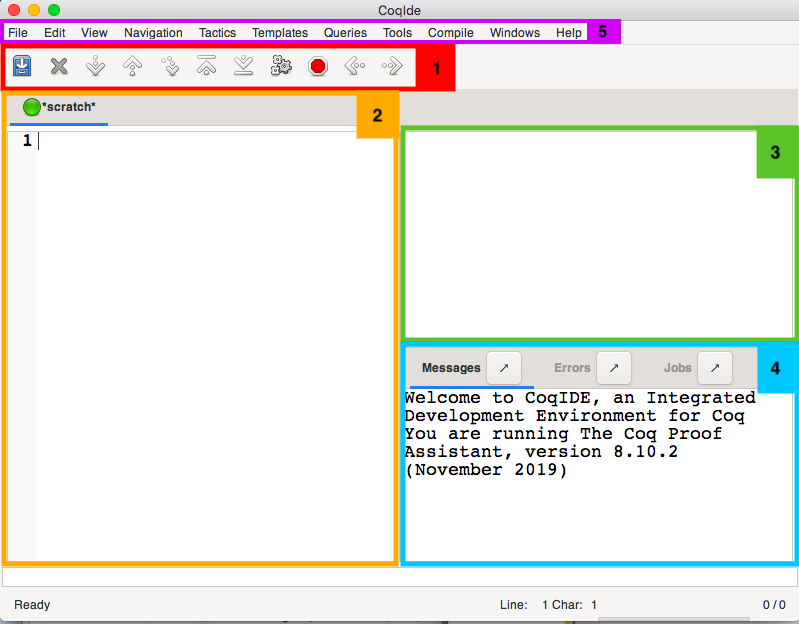
\includegraphics[width=\textwidth]
        {CoqScreenshots/CoqIDEv8_10_2_color.png}}
        \label{fig:IDEcolor} 
        \captionof{figure}{CoqIDE v8.10.2  
        (1) Toolbar. (2) Script Buffer. (3) Goal Window. (4) Message Window. }
\end{minipage}

\subsubsection{Toolbar for CoqIDE v8.10.2}
\hspace{-0.75cm}
\begin{tabular}{ C L }
\centered{
\includegraphics[width=\iconsize]
        {CoqScreenshots/save_10.png}}
        & \centeredl{Save current buffer. 
        If it hasn't been previously saved, functions as save as; use the extension .v to save as a Coq file.
        } \\ \\
\centered{
\includegraphics[width=\iconsize]
        {CoqScreenshots/close_10.png}}
	& \centeredl{Close current buffer. 
	Gives a warning if the file has unsaved changes.
	} \\ \\
\centered{
\includegraphics[width=\iconsize]
        {CoqScreenshots/step_forward_10.png}}
	& \centeredl{Forward one command.
	Steps forward to evaluate the next command in the current file.
	} \\ \\
\centered{
\includegraphics[width=\iconsize]
        {CoqScreenshots/step_backward_10.png}}
	& \centeredl{Backward one command.
	Steps backward one command in the file, returns the state to where it was before evaluating that command. 
	} \\ \\ 
\centered{
\includegraphics[width=\iconsize]
        {CoqScreenshots/go_to_cursor_10.png}}
	& \centeredl{Go to cursor.
	Evaluate all commands in file up to where the cursor currently is.
	} \\ \\ 
\centered{
\includegraphics[width=\iconsize]
        {CoqScreenshots/go_to_top_10.png}}
	& \centeredl{Restart Coq.
	Returns to the top of the file, where no commands have been evaluated.
	} \\ \\ 
\centered{
\includegraphics[width=\iconsize]
        {CoqScreenshots/go_to_bottom_10.png}}
	& \centeredl{Go to end.
	Evaluate to the bottom of the file. 
	Does not work as well with load commands and require import commands.
	} \\ \\
\centered{
\includegraphics[width=\iconsize]
        {CoqScreenshots/check_10.png}}
	& \centeredl{Fully check the document.
	Submits proof terms to the Coq kernel for type checking.
	} \\ \\
\centered{
\includegraphics[width=\iconsize]
        {CoqScreenshots/stop_10.png}}
	& \centeredl{Interrupt computations.
	Stops computation at whatever point was reached before pressing the button.
	} \\ \\
\centered{
\includegraphics[width=\iconsize]
        {CoqScreenshots/next_occurrence_10.png}}
	& \centeredl{Next Occurrence.
	Goes to the next occurrence of whatever the cursor is currently by. 
	Works well for longer words.
	} \\ \\
\centered{
\includegraphics[width=\iconsize]
        {CoqScreenshots/previous_occurrence_10.png}}
	& \centeredl{Previous Occurrence.
	Goes to the previous occurrence of whatever the cursor is currently by.
	Works well for longer words.
	}
\end{tabular}









\subsection{Script Buffer}
Here you can type out new definitions and proofs in a new buffer, or open a buffer from a saved file by going to the File tab $\to$ Open, then choosing the file. 
You can edit and save new and existing buffers here. 
\begin{code} 
	This block represents a script buffer in this tutorial. 
\end{code}



\subsection{Goal Window}
Goals to be proven will be displayed here. 
This window will be empty unless you're in a proof environment; inside the proof environment, it will display what you goal are currently proving, what goals are left to be proved, or that there are no more subgoals and your proof is complete.
\begin{goal} 
	This block represents the goal window in this tutorial. 
\end{goal}



\subsection{Message Window}
Any messages resulting from an executed command will be displayed here. 
Results from queries are also printed out here. 
Clicking the arrow in the corner of the Messages, Errors, or Jobs tab here will create a separate window for that tab. 
When the separate window is closed, it will return to the main Coq IDE window. 
\begin{msg} 
	This block represents the message window in this tutorial. 
\end{msg}

















\newpage
\section{The Gallina Specification Language}
	\label{Sec: gallina}
	




Gallina is the specification language of Coq. 
It is a functional language, fairly similar to \href{https://en.wikipedia.org/wiki/OCaml}{OCaml} or 
\href{https://en.wikipedia.org/wiki/Standard_ML}{SML} if you are familiar with those. 
It includes things such as pattern matching, let-in definitions, and recursive functions. 

~\\
The reference manual for the Gallina Language Specification can be found here: 
\\ 
\url{https://coq.inria.fr/distrib/current/refman/language/gallina-specification-language.html#}

~\\ 
This details the grammar of the language; 
lexical conventions (i.e. keywords, formatting of identifiers/variables, etc.); 
the syntax of terms; types; etc; then goes into the grammar of The Vernacular (the language of commands of Gallina). 
If you are familiar with programming language basics like these, you may find this of interest 
and it could be beneficial to you; if not, it may be a bit confusing 

~\\
A few important things to note about the Vernacular of Gallina are that each sentence begins with a capital letter and ends 
with a dot (i.e. period), and whitespace is used to separate terms but otherwise ignored.

~\\ 
Starting in the 
\href{https://coq.inria.fr/distrib/current/refman/language/gallina-specification-language.html#assumptions}
{Assumptions}
section, there are some examples mixed in with the formal command definitions 
and syntax specifications for their use, which may be beneficial if you are struggling with a particular command 
and need more information beyond what this tutorial provides. 












	
~\\~\\
\section{The Calculus of Inductive Constructions}
	\label{Sec: calculus}
	
The reference manual for the Calculus of Inductive Constructions used by Coq can be found here:
\\
\url{https://coq.inria.fr/distrib/current/refman/language/cic.html#calculusofinductiveconstructions}

~\\
This gives things such as typing rules, conversion rules, subtyping rules, inductive definitions, etc., 
used by Coq. 

~\\
This is useful if you'd like a more in-depth perspective on the formal definitions and intuition behind 
the typing system in Coq - but it is not necessary to know or understand these definitions in great 
detail to have Coq be of use to you. 

~\\
This will not be discussed further in this tutorial to keep things simple. 
Please see the website given above if this is of interest to you. 










	

\newpage
\part{Functional Programming in Coq}
	\label{Part: program}
\section{Coq Basics}
	\label{Sec: basics}
	
The language of Coq is functional, and has similarities to OCaml. If you are not familiar with functional programming, this section will help introduce some basic syntax and concepts to get you started. See file ``Basics.v"

\subsection{Comments} \label{comments}
Comments in Coq are surrounded by (*  *).
\begin{code}
	\cmt{ This is a comment in Coq. }
\end{code}


\subsection{Commands} \label{commands}
All commands in Coq must end with a period. The various available commands are discussed throughout this document; please see the respective sections for more information on any specific commands.


\subsection{Pattern Matching} \label{pattern_matching}

Pattern matching is a useful way to specify what should occur when you see a specific option of a type. For example, with booleans you have the options of true and false.
In general, you have something like this for a single variable:

\hspace{-1cm}
\begin{tabular}{p{8cm} p{8cm}}
\begin{code}
	\match var \with 			\\
	$\mid$ opt1 $=>$ expr1		\\
	$\mid$ opt2 $=>$ expr2		\\
	\End
\end{code}
&
\begin{code}
	\match b \with 				\\
	$\mid$ true $=>$ false		\\
	$\mid$ false $=>$ true		\\
	\End
\end{code}
\end{tabular}

and something like this if you'd like to match over a combination of variables:

\begin{code}
	\match (var1, var2) \with 					\\
	$\mid$ (var1opt1, var2opt1) $=>$ expr1		\\
	$\mid$ (var1opt2, var2opt2) $=>$ expr2		\\
	$\mid$ ...	$=>$ ...						\\
	$\mid$ (\_\ , \_ ) $=>$ exprX				\\
	\End
\end{code}

\noindent
The underscore in the last option allows you to specify only the options that you care about at the top, and then for all other cases, do \blue{exprX}. The underscore is not necessary if you've listed all possible options or combinations of options as possible matches.

~\\ \noindent
See example \ref{bool_ops} for some simple boolean functions using pattern matching.





\subsection{Lists} \label{list} 
Coq has built in notation for lists that you can use; however, to use the notations, you must make sure to load the List library beforehand. 
\begin{code}
	\Load List.
\end{code}


\noindent
Lists cannot contain elements of different types. 
If you want to have a list with different types, you must first create a new user-defined type (see defining Inductive objects, section \ref{inductive}) or use a tuple (see \ref{tuple}).
From there, you can use the following notations (general case on the left, list of numbers on the right):
\hspace{-1cm}
\begin{tabular}{p{8cm} p{8cm}}
\begin{code}
	v1::v2:: ... ::[\ ]
\end{code}
\begin{code}
	[ v1; ...; vN ]
\end{code}
&
\begin{code}
	1::2::3::4::5::6::7::8::9::0::[\ ]
\end{code}
\begin{code}
	[ 1; 2; 3; 4; 5; 6; 7; 8; 9; 0 ]
\end{code} 
\end{tabular}
The empty list is always denoted as [ ]; When using the double colon appended list, you must have the empty list as the right-most element.


\noindent
You can also define your own lists like they are defined in Coq; for example, this defines a list of nat numbers:
\begin{code}
\Inductive \nm{natlist} : \Type :=
  $\mid$ nil
  $\mid$ cons (n : nat) (l : natlist).
\end{code}







~\\ ~\\
\noindent
The following functions are defined in the List library; for examples of the use of most of these, please see Example \ref{list}.

\begin{tabular}{r L}
length :	
	& number of elements in list 				 \\
head : 
	& first element (with default) 				\\
tail : 
	& all but first element						\\
app : 
	& concatenation						\\
rev : 
	& reverse								\\
nth : 
	& accessing n-th element (with default)		\\
map : 
	& applying a function						\\
flat\_map : 
	& applying a function returning lists			\\
fold\_left : 
	& iterator (from head to tail)				\\
fold\_right : 
	&iterator (from tail to head)
\end{tabular}



\subsection{Tuples} \label{tuple} 

A tuple is given by two or more comma separated objects enclosed in parentheses. Tuples can contain items of the same or different types.

\hspace{-1cm}
\begin{tabular}{p{8cm} p{8cm}}
\begin{code}
	(v1, ..., vN)
\end{code}
&
\begin{code}
	(1, 2, 3)
\end{code}
\end{tabular}



\subsection{Boolean Expressions for Branches} \label{bool_expr} 
To use boolean expressions on numbers in an if then else, make sure you've imported Arith and loaded Bool:
\begin{code}
	\cmd{Require Import} Arith.	\\
	\Load Bool.
\end{code}

Checking less than:
\begin{code}
	x $<?$ y 
\end{code}

Checking equal to:
\begin{code}
	x $=?$ y
\end{code}

Checking less than or equal to:
\begin{code}
	x $<=?$ y
\end{code}

\noindent
To my knowledge, there is not pre-defined notation in Coq for greater than or not equal operations - however, you can get around this fairly easily by defining the functionality and notations yourself  (see Example \ref{bool_expr}).






\subsection{Option Types} \label{opt_ty}
When using some built-in functions in Coq, you may come across option types. 
Option types are particularly useful when you want to return an element if it is found, or be told explicitly that it does not exist.
In other languages, you would either need to have two separate functions, one to check if it exists and one to obtain the value, or return some sort of 'neutral' value, like -1 or 0, to indicate an item wasn't found.
Option types are defined as: 

\begin{code} 
	\Inductive \nm{option} (A : \Type) : \Type :=	\\ \-\ \quad
	$\mid$ None : option A					\\ \-\ \quad
	$\mid$ Some : A $->$ option A
\end{code}

and an example of it being used:

\begin{code}
	\Fixpoint \nm{at\_n} (n : nat) (l : Datatypes.list nat) : option nat :=	\\ \-\ \quad
	  \match l \with 										\\ \-\ \qquad
	  $\mid$ [ ] $=>$ None								\\ \-\ \qquad
	  $\mid$ hd :: tl $=>$  \If (n $=?$ 0)			\\ \-\ \qquad\qquad\qquad\quad
		    \Then Some hd					\\ \-\ \qquad\qquad\qquad\quad
		    \Else at\_n (n - 1) tl							\\ \-\ \qquad
	  \End.
\end{code}

\noindent
In this function, we are recursively going through the list to find the item at position n in the list.
To do this, at each iteration we are checking if we have found the empty list, if so we return None; 
otherwise we pull apart the head element of the list from the tail of the list, and if n is 0, then we return Some with that head element; 
if n is greater than 0, then we make the recursive call on n -1 and the tail of the list. 
The function will execute until we either find the empty list or the element at position n.
We can then use pattern matching on the option type to obtain and use the value that was found or do something else having found that the value doesn't exist.











\newpage
\section{Using External Files/Libraries}
	\label{Sec: files}
	

\subsection{Standard Libraries} \label{stdlib}

\begin{tabular}{l L}
\TT{Logic} 	&
	Classical logic and dependent equality
\\	
\TT{Arith}		&
	Basic Peano arithmetic
\\
\TT{PArith} 	&
	Basic positive integer arithmetic
\\
\TT{NArith}  	&
	Basic binary natural number arithmetic
\\
\TT{ZArith} 	&
	Basic relative integer arithmetic
\\
\TT{Numbers} 	&
	Various approaches to natural, integer and cyclic numbers (currently axiomatically and on top of $2^{31}$ binary words)
\\
\TT{Bool} 		&
	Booleans (basic functions and results)
\\
\TT{Lists}�		& 
	Monomorphic and polymorphic lists (basic functions and results), Streams (infinite sequences defined with co-inductive types)
\\
\TT{Sets}		& 
	Sets (classical, constructive, finite, infinite, power set, etc.)
\\
\TT{FSets}�		&
	Specification and implementations of finite sets and finite maps (by lists and by AVL trees)
\\
\TT{Reals}		&
	Axiomatization of real numbers (classical, basic functions, integer part, fractional part, limit, derivative, Cauchy series, power series and results,...)
\\
\TT{Relations}		&
	Relations (definitions and basic results)
\\
\TT{Sorting}		&
	Sorted list (basic definitions and heapsort correctness)
\\
\TT{Strings}�		&
	8-bits characters and strings
\\
\TT{Wellfounded}		&
	Well-founded relations (basic results)
\\
\end{tabular}




\subsection{Require} \label{require}
To use the standard libraries or other compiled files, you first need to tell the environment that it needs to load the compiled file. 
\TT{Require} adds the specified module and all of its dependencies to the environment. 

\begin{code}
	\cmd{Require} Logic.
\end{code}

\noindent
\TT{Require Import} loads the specified module and its dependences, then imports the contents of the specified module.

\begin{code}
	\cmd{Require Import} Bool.
\end{code}

\noindent
\TT{Require Export} acts like \TT{Require Import}, but will ensure that any module B that uses \TT{Require Import} on the module A that contained the \TT{Require Export} command will import both module A and the one specified in the \TT{Require Export} command.

\begin{code}
	\cmd{Require Export} Bool.
\end{code}




\subsection{Load} \label{load}
This is used to load a file or library into the current environment. 
To load one of the standard libraries, you can simply use the \TT{Load} command.

\begin{code}
	\cmd{Load} Arith.
\end{code}

\noindent
However, to load any other existing file, you will likely need to specify where to look for the file; to do this, there is the 
\TT{Add LoadPath} command.
All the commands in the loaded file will be evaluated

\begin{code}
	\cmd{Add} LoadPath \str{``/myDirectory/path/"}. \\
	\cmd{Load} myFile. 
\end{code}











\newpage
\section{Defining in Coq}
	\label{Sec: defining}
	
Please see file ``Defining.v" to follow along with this code in the CoqIDE. 

\subsection{Sorts} \label{subsec: sort}
There are three main Sorts for defining types: {\bf Prop}, {\bf Set}, and {\bf Type}. 
\begin{itemize}
	\item {\bf Prop}: This type is for logical propositions. 
	\item {\bf Set}: This type is for small sets, such as booleans (bool) and natural numbers (nat). 
	\item {\bf Type}: This type can be used for small sets as well as larger sets - it encompasses both {\bf Prop} and {\bf Set}. 
\end{itemize}

\noindent
These are used in defining Inductive types, as shown in the next section.




\subsection{Inductive} \label{subsec: inductive}
The command Inductive is used to define simple inductive types and the constructors used in the type. 
The name is placed directly after the keyword Inductive, when a colon followed by the Sort 
(discussed in the previous section) of the inductive type you are defining. 
This is followed by $:=$ and the constructors (i.e. elements) included in that type.  
For example, boolean values are defined in Coq as follows:

\hspace{-1cm}
\begin{tabular}{p{8cm} p{8cm}}
	\begin{code}
		\df{Inductive} \nm{bool} : \ty{Set} := 	\\ \-\ \quad
 		 $\mid$ true						\\ \-\ \quad
 		 $\mid$ false.						\\		
	\end{code}
&
	\begin{msg}
		bool is defined			\\
		bool\_rect is defined		\\
		bool\_ind is defined		\\
		bool\_rec is defined
	\end{msg}
\end{tabular}

\noindent
and nat numbers are defined as:

\hspace{-1cm}
\begin{tabular}{p{8cm} p{8cm}}
	\begin{code}
		\df{Inductive} \nm{nat} : \ty{Set} := 		\\ \-\ \quad
 		 $\mid$ O	: nat						\\ \-\ \quad
 		 $\mid$ S : nat $->$ nat.				\\		
	\end{code}
&
	\begin{msg}
		nat is defined			\\
		nat\_rect is defined		\\
		nat\_ind is defined		\\
		nat\_rec is defined
	\end{msg}
\end{tabular}

\noindent
You can see what all the definitions it created are by using Print:

\begin{code}	\cmd{Print} nat.			\end{code}
\begin{msg}
	\df{Inductive} nat : \ty{Set} :=  O : \nm{nat} $\mid$ S : \nm{nat} $->$ \nm{nat}
\end{msg}
\begin{code}	\cmd{Print} nat\_rect.		\end{code}
\begin{msg}
	nat\_rect = 	\\
	\kw{fun} (P : \nm{nat} $->$ \ty{Type}) (f : P \nm{O}) (f0 : \kw{forall} n : \nm{nat}, P n $->$ P (\nm{S} n)) $=>$	\\
	\kw{fix} F (n : \nm{nat}) : P n := \kw{match} n \kw{as} n0 \kw{return} (P n0) \kw{with}		\\ \-\ \qquad\qquad
			$\mid$ \nm{O} $=>$ f									\\ \-\ \qquad\qquad
			$\mid$ \nm{S} n0 $=>$ f0 n0 (F n0)							\\ \-\ \qquad\qquad
			\kw{end}												\\ \-\ \qquad
		: \kw{forall} P : \nm{nat} $->$ \ty{Type}, P \nm{O} $->$ (\kw{forall} n : \nm{nat}, P n 
			$->$ P (\nm{S} n)) $->$ \kw{forall} n : \nm{nat}, P n
	\\ \\
	Argument scopes are [function\_scope \_ function\_scope \_\ ]
\end{msg}
\begin{code}	\cmd{Print} nat\_ind.		\end{code}
\begin{msg}
	nat\_rect = 	\\
	\kw{fun} (P : \nm{nat} $->$ \ty{Prop}) (f : P \nm{O}) (f0 : \kw{forall} n : \nm{nat}, P n $->$ P (\nm{S} n)) $=>$	\\
	\kw{fix} F (n : \nm{nat}) : P n := \kw{match} n \kw{as} n0 \kw{return} (P n0) \kw{with}		\\ \-\ \qquad\qquad
			$\mid$ \nm{O} $=>$ f									\\ \-\ \qquad\qquad
			$\mid$ \nm{S} n0 $=>$ f0 n0 (F n0)							\\ \-\ \qquad\qquad
			\kw{end}												\\ \-\ \qquad
		: \kw{forall} P : \nm{nat} $->$ \ty{Prop}, P \nm{O} $->$ (\kw{forall} n : \nm{nat}, P n 
			$->$ P (\nm{S} n)) $->$ \kw{forall} n : \nm{nat}, P n
	\\ \\
	Argument scopes are [function\_scope \_ function\_scope \_\ ]
\end{msg}
\begin{code}	\cmd{Print} nat\_rec.		\end{code}
\begin{msg}	
	nat\_rec = 								\\
	\kw{fun} P : \nm{nat} $->$ \ty{Set} $=>$ \nm{nat\_rect} P				\\ \-\ \qquad
		: \kw{forall} P : \nm{nat} -$>$ \ty{Set},					
		  P \nm{O} $->$						
       			(\kw{forall} n : \nm{nat}, P n $->$ P (\nm{S} n)) $->$ \kw{forall} n : \nm{nat}, P n 
	\\ \\
	Argument scopes are [function\_scope \_ function\_scope \_\ ]
\end{msg}

\noindent
You can use these properties of what you've defined in proofs.

~\\
\noindent
Similarly, you can define days of the week:

\hspace{-1cm}
\begin{tabular}{p{8cm} p{8cm}}
\begin{code}
\Inductive \nm{day}: \Type :=	\\ \-\quad
 $\mid$ monday : day		\\ \-\quad
 $\mid$ tuesday : day		\\ \-\quad
 $\mid$ wednesday : day		\\ \-\quad
 $\mid$ thursday : day		\\ \-\quad
 $\mid$ friday : day			\\ \-\quad
 $\mid$ saturday : day		\\ \-\quad
 $\mid$ sunday : day.
\end{code}
&
\begin{msg}			
day is defined			\\
day\_rect is defined		\\
day\_ind is defined		\\
day\_rec is defined		
\end{msg}
\end{tabular}

\noindent
or lists:

\hspace{-1cm}
\begin{tabular}{p{8cm} p{8cm}}
\begin{code}
\Inductive \nm{list} (A: \ty{Set}) : \ty{Set} :=	\\ \-\ \quad
$\mid$ nil : list A						\\ \-\ \quad
$\mid$ cons : A $->$ list A.				\\
\end{code}
&
\begin{msg}
list is defined			\\
list\_rect is defined		\\
list\_ind is defined		\\
list\_rec is defined		
\end{msg}
\end{tabular}







\subsection{Definition} \label{subsec: definition}

The command Definition is used to bind an name to some term. 
The name is always placed directly after the keyword Definition, 
and the term to bind to the name is given after $:=$. 
For example, we can give the name $x$ a simple value of 4: 

\hspace{-1cm}
\begin{tabular}{p{8cm} p{8cm}}
\begin{code}
Definition x := 4.
\end{code}
& 
\begin{msg}
x is defined
\end{msg}
\end{tabular}

\noindent
or we can use this to define functions, such as the following simple function 
(using the previous weekday inductive type definition), 
taking a weekday as input and giving back the weekday as output. 
Here, we are specifying the parameter $d$ of type $day$ must be given to the function. 
When giving a parameter, you give the $(paramName: type)$ as in $(d:day)$. 
The parameters are then followed by the return type, as in $: returnType$. 
This is shown in the following example. 

\hspace{-1cm}
\begin{tabular}{p{8cm} p{8cm}}
\begin{code}
\Definition \nm{next\_weekday} (d:day) : day :=	\\ \-\ \quad
  \match d \with							\\ \-\ \qquad
   $\mid$ monday $=>$ tuesday				\\ \-\ \qquad
   $\mid$ tuesday $=>$ wednesday			\\ \-\ \qquad
   $\mid$ wednesday $=>$ thursday			\\ \-\ \qquad
   $\mid$ thursday $=>$ friday				\\ \-\ \qquad
   $\mid$ friday $=>$ monday				\\ \-\ \qquad
   $\mid$ saturday $=>$ monday			\\ \-\ \qquad
   $\mid$ sunday $=>$ monday				\\ \-\ \quad
  \End.
\end{code}
& 
\begin{msg}
next\_weekday is defined
\end{msg}
\end{tabular}

\noindent
Another simple example function definition 
(using the previous nat number inductive type definition) 
is taking a nat number and returning that result of adding 2 to that nat number: 

\hspace{-1cm}
\begin{tabular}{p{8cm} p{8cm}}
\begin{code}
\Definition \nm{plus2} (n:nat) : nat :=		\\ \-\ \quad
  \match n \with						\\ \-\ \qquad
    $\mid$ O $=>$ S (S O)				\\ \-\ \qquad
    $\mid$ \_ $=>$ S (S n)				\\ \-\ \quad
  \End.
\end{code}
& 
\begin{msg}
plus2 is defined
\end{msg}
\end{tabular}

\noindent
You can also give multiple parameters, as shown in the example below using 3 parameters: 

\hspace{-1cm}
\begin{tabular}{p{12cm} p{4cm}}
\begin{code}
\Definition \nm{choose1} (b: bool) (n1: Datatypes.nat) (n2: Datatypes.nat) : Datatypes.nat :=	\\ \-\ \quad
  \match b \with										\\ \-\ \qquad
    $\mid$ true $=>$ n1								\\ \-\ \qquad
    $\mid$ false $=>$ n2								\\ \-\ \quad
  \End.
\end{code}
& 
\begin{msg}
choose1 is defined
\end{msg}
\end{tabular}

\noindent
We have to specify that we would like to use Datatypes.nat as our type in order to use 
natural numbers (i.e. 0, 1, 2, 3, 4, 5, 6, 7, 8, 9), as we have not specified how to interpret these 
numbers from our definition of nat (you can do this using the Notation command 
- using this command will be discussed in the following subsection \ref{subsec: notation}). 
Alternately, we can define the same function without giving the types of the parameters 
(however, it is always best practice to declare the types of all parameters, 
to ensure they are interpreted as you expect them to be). 
When you do not specify the types of parameters, the parentheses around the 
parameter names are optional. 

\hspace{-1cm}
\begin{tabular}{p{12cm} p{4cm}}
\begin{code}
\Definition \nm{choose1$'$} b n1 n2 : Datatypes.nat :=		\\ \-\ \quad
  \match b \with										\\ \-\ \qquad
    $\mid$ true $=>$ n1								\\ \-\ \qquad
    $\mid$ false $=>$ n2								\\ \-\ \quad
  \End.
\end{code}
& 
\begin{msg}
choose1$'$ is defined
\end{msg}
\end{tabular}

\noindent
Both {\it $choose$1} and {\it $choose$1$'$} have the same functionality. 






\subsection{Notation} \label{subsec: notation}






\subsection{Fixpoint} \label{subsec: fixpoint}






\subsection{Compute} \label{subsec: compute}










\newpage
\section{Examples: Programming in Coq}
	\label{Sec: program examples}
	
\subsection{Cards} \label{cards}

Please see the ``cards.v'' file to follow along with this example. 

\noindent
This is a simple example defining suits and values for cards, and what a valid card is. In the function \TT{check\_num}, we check if the number given is less than 11 and greater than 1. In function \TT{is\_valid\_card}, we pattern match against various types of cards. Here, the given card is represented by the variable x. The type card is defined to be \TT{c (s: suit) (v: val)}, and we know that an \TT{s} of type suit can only be one of the valid suits we defined, so we can use some variable, say \TT{q}, to represent allowing any suit type; the part we need to ensure is valid is the value given to the suit, since a valid card can only have a value of an ace, king, queen, jack, or number values 2 thru 10.

\begin{code}
\Load List. 	\\
\Load Bool.
\\ \\
\Inductive \nm{suit} : \Type :=
  $\mid$ heart
  $\mid$ diamond
  $\mid$ spade
  $\mid$ club.

\Inductive \nm{val} : \Type :=
  $\mid$ ace
  $\mid$ king
  $\mid$ queen
  $\mid$ jack
  $\mid$ num (n: nat).

\Inductive \nm{card} : \Type :=
  $\mid$ c (s: suit) (v: val).
\\ \\
\cmt{Card: 2 of Spades} 	\\
\Check (c spade (num 2)).
\\ \\
\cmt{List of suits}	\\
\Check (ace::king::[ ]).
\\ \\
\cmt{List of Cards} 	\\
\Check [c heart ace; c diamond king; c spade queen].
\\ \\
\Definition \nm{check\_num} (x: nat) : bool :=	 \\ \-\ \quad
  \If (x $<?$ 11)						 \\ \-\ \quad
  \Then \If (1 $<?$ x)					 \\ \-\ \qquad
       \Then true						 \\ \-\ \qquad
       \Else false						 \\ \-\ \quad
  \Else false.
%\\ \\
%Compute check\_num 0.
%Compute check\_num 1.
%Compute check\_num 2.
%Compute check\_num 10.
%Compute check\_num 11.
\\ \\
\Definition \nm{is\_valid\_card} (x: card) : bool :=	 \\ \-\ \quad
 \match x \with						 \\ \-\ \quad
  $\mid$ c q ace $=>$ true				 \\ \-\ \quad
  $\mid$ c q king $=>$ true			 \\ \-\ \quad
  $\mid$ c q queen $=>$ true			 \\ \-\ \quad
  $\mid$ c q jack $=>$ true			 \\ \-\ \quad
  $\mid$ c q (num n) $=>$ 				 \\ \-\ \qquad\quad
        \If (check\_num n)				 \\ \-\ \qquad\quad
        \Then true			 			 \\ \-\ \qquad\quad
        \Else false						 \\ \-\ \quad
 \End.
\\ \\
\cmt{Ace of Hearts is a valid card}	\\
Compute is\_valid\_card (c heart ace).
\\ \\
\cmt{11 of Diamonds is NOT a valid card}	\\
Compute is\_valid\_card (c diamond (num 11)).

%Compute is\_valid\_card (c heart (num 10)).
%Compute is\_valid\_card (c heart king).
%Compute is\_valid\_card (c heart queen).
%Compute is\_valid\_card (c heart jack).
%Compute is\_valid\_card (c heart (num 9)).
%Compute is\_valid\_card (c heart (num 1)).
%\Check (c heart ace).

\end{code}














\newpage
\subsection{Boolean Operations} \label{bool_ops}

Please see the ``bool.v'' file to follow along with this example. 

\noindent
This is a simple example of the definition of booleans and some boolean operations.

\begin{code}
\Inductive \nm{bool} :=
  $\mid$ true
  $\mid$ false.
\\ \\
\Definition \nm{not} (b : bool) : bool :=		\\ \-\ \quad
  \match b \with							\\ \-\ \quad
   $\mid$ true $=>$ false					\\ \-\ \quad
   $\mid$ false $=>$ true					\\ \-\ \quad
  \End.
\\ \\
\Definition \nm{and} (b1 b2 : bool) : bool :=	\\ \-\ \quad
  \match (b1, b2) \with					\\ \-\ \quad
   $\mid$ (true, true) $=>$ true				\\ \-\ \quad
   $\mid$ (\_\ , \_\ ) $=>$ false				\\ \-\ \quad
  \End.
\\ \\
\Definition \nm{or} (b1 b2 : bool) : bool :=		\\ \-\ \quad
  \match (b1, b2) \with					\\ \-\ \quad
   $\mid$ (false, false) $=>$ false			\\ \-\ \quad
   $\mid$ (\_\ , \_\ ) $=>$ true				\\ \-\ \quad
  \End.
\\ \\
\Definition \nm{xor} (b1 b2 : bool) : bool :=		\\ \-\ \quad
  \match (b1, b2) \with					\\ \-\ \quad
   $\mid$ (true, false) $=>$ true				\\ \-\ \quad
   $\mid$ (false, true) $=>$ true				\\ \-\ \quad
   $\mid$ (\_\ , \_\ ) $=>$ false				\\ \-\ \quad
  \End.
\end{code}




\newpage
\subsection{Boolean Expressions for Branches} \label{bool_expr}

Please see the ``bool\_expr.v'' file to follow along with this example. 

\noindent 
This is a simple example defining less than, equal to, and less than or equal to operations over numbers.

\begin{code}
	\cmd{Require Import} Arith.	\\
	\Load Bool.
	\\ \\
	\Definition \nm{lt} (n m : nat) : bool :=		\\ \-\ \qquad
		  \If (n $<?$ m)					\\ \-\ \qquad
		  \Then true					\\ \-\ \qquad
		  \Else false.					\\
	\Notation \str{``n $<$ m"} := (lt n m).
	\\ \\
	\Definition \nm{gt} (n m : nat) : bool :=	\\ \-\ \qquad
		  \If (m $<?$ n)					\\ \-\ \qquad
		  \Then true					\\ \-\ \qquad
		  \Else false.					\\
	\Notation \str{``n $>$ m"} := (gt n m).
	\\ \\
	\Definition \nm{eq} (n m : nat) : bool :=	\\ \-\ \qquad
		  \If (n $=?$ m)					\\ \-\ \qquad
		  \Then true					\\ \-\ \qquad
		  \Else false.					\\
	\Notation \str{``n $=$ m"} := (eq n m).
	\\ \\
	\Definition \nm{neq} (n m : nat) : bool :=	\\ \-\ \qquad
		  \If (n $=?$ m)					\\ \-\ \qquad
		  \Then false					\\ \-\ \qquad
		  \Else true.					
	\\ \\
	\Definition \nm{lteq} (n m : nat) : bool :=	\\ \-\ \qquad
		  \If (n $<=?$ m)				\\ \-\ \qquad
		  \Then true					\\ \-\ \qquad
		  \Else false.					\\
	\Notation \str{``n $<=$ m"} := (lteq n m).					
	\\ \\
	\Definition \nm{gteq} (n m : nat) : bool :=	\\ \-\ \qquad
		  \If (m $<=?$ n)				\\ \-\ \qquad
		  \Then true					\\ \-\ \qquad
		  \Else false.					\\
	\Notation \str{``n $>=$ m"} := (gteq n m).
\end{code}













\newpage
\subsection{Days of the Week} \label{days}

Please see file ``days.v'' to follow along with this example. 

~\\
This example is fairly simple, giving some basic definitions and functions, and showing a use of a tuple in Coq.  

~\\
\noindent
First, we define what a day is using the following definition:

\begin{code}
\Inductive \nm{day}: \Type :=		\\ \-\ \quad
  $\mid$ monday : day			\\ \-\ \quad
  $\mid$ tuesday : day			\\ \-\ \quad
  $\mid$ wednesday : day			\\ \-\ \quad
  $\mid$ thursday : day			\\ \-\ \quad
  $\mid$ friday : day				\\ \-\ \quad
  $\mid$ saturday : day			\\ \-\ \quad
  $\mid$ sunday : day.
\end{code}

\noindent
Then we define a simple function to compute what the next weekday is after a given day. 
This takes a day as input, and gives back what the next weekday would be.

\begin{code}
\Definition \nm{next\_weekday} (d:day): day :=		\\ \-\ \quad
  \match d \with								\\ \-\ \qquad
   $\mid$ monday $=>$ tuesday					\\ \-\ \qquad
   $\mid$ tuesday $=>$ wednesday				\\ \-\ \qquad
   $\mid$ wednesday $=>$ thursday				\\ \-\ \qquad
   $\mid$ thursday $=>$ friday					\\ \-\ \qquad
   $\mid$ friday $=>$ monday					\\ \-\ \qquad
   $\mid$ saturday $=>$ monday				\\ \-\ \qquad
   $\mid$ sunday $=>$ monday					\\ \-\ \quad
  \End.
\end{code}

\noindent
We can perform some simple computations to check the correctness of our function:

\hspace{-1cm}
\begin{tabular}{p{9cm} p{7cm}}
\begin{code} 	Compute (next\_weekday friday).	\end{code}
\begin{code}	Compute next\_weekday (next\_weekday friday).	\end{code}	
&	
\begin{msg}	     = \nm{monday}     : \nm{day}	\end{msg}
\begin{msg}	     = \nm{tuesday}     : \nm{day}		\end{msg}
\end{tabular}

\noindent
To make this a bit more interesting, we can also define some other things, such as sports:

\begin{code}
\Inductive \nm{sport}: \Type :=		\\ \-\ \quad
  $\mid$ tennis : sport			\\ \-\ \quad
  $\mid$ basketball : sport			\\ \-\ \quad
  $\mid$ baseball : sport 			\\ \-\ \quad
  $\mid$ cricket : sport			\\ \-\ \quad
  $\mid$ football : sport			\\ \-\ \quad
  $\mid$ dance : sport			\\ \-\ \quad
  $\mid$ gymnastics : sport		\\ \-\ \quad
  $\mid$ run : sport				\\ \-\ \quad
  $\mid$ rugby : sport			\\ \-\ \quad
  $\mid$ weights : sport			\\ \-\ \quad
  $\mid$ swim : sport.
\end{code}

and activities: 

\begin{code}
\Inductive \nm{activity}: \Type :=	\\ \-\ \quad
  $\mid$ class : activity			\\ \-\ \quad
  $\mid$ lab : activity				\\ \-\ \quad
  $\mid$ meeting : activity			\\ \-\ \quad
  $\mid$ seminar : activity			\\ \-\ \quad
  $\mid$ volunteer : activity		\\ \-\ \quad
  $\mid$ club : activity			\\ \-\ \quad
  $\mid$ work : activity.	
\end{code}

\noindent
Now, it is possible to create a function that returns a schedule for each day, 
consisting of a tuple of an activity and a sport. 

\begin{code}
\Definition \nm{daily\_schedule} (d:day): activity * sport :=		\\ \-\ \quad
  \match d \with										\\ \-\ \qquad
   $\mid$ monday $=>$ (meeting, run)					\\ \-\ \qquad
   $\mid$ tuesday $=>$ (class, tennis)					\\ \-\ \qquad
   $\mid$ wednesday $=>$ (seminar, baseball)				\\ \-\ \qquad
   $\mid$ thursday $=>$ (class, rugby)					\\ \-\ \qquad
   $\mid$ friday $=>$ (lab, dance)						\\ \-\ \qquad
   $\mid$ saturday $=>$ (club, swim)						\\ \-\ \qquad
   $\mid$ sunday $=>$ (volunteer, basketball)				\\ \-\ \quad
  \End.	
\end{code}

\noindent
Of course, it is also possible to create more complex schedules, but this 
should give you an the basic idea of how to do that. 










\newpage
\subsection{List} \label{list}

A simple example to demonstrate some uses of the built-in lists and list functions, and define a search function for lists of nat numbers. To use the notations and functions, you'll want to load List and open the list\_scope so everything works properly.

\begin{code}
	\cmd{Require Import} \nm{Arith}.				\\
	\cmd{Load} List. 							\\
	\cmd{Open Scope} list\_scope.					\\
	\\
	\Fixpoint \nm{search} (l : Datatypes.list nat) (n: nat) : bool :=  	\\ \-\ \quad
	  \match l \with 								\\ \-\ \qquad
	   $\mid$ [ ] $=>$ false						\\ \-\ \qquad
	   $\mid$ hd :: tl $=>$ 						\\ \-\ \qquad\qquad
	      \If (n $=?$ hd)							\\ \-\ \qquad\qquad
	      \Then true								\\ \-\ \qquad\qquad
	      \Else search tl n							\\ \-\ \quad
	  \End.									
\end{code}

\noindent
Uses of the list functions and results:
	  
\hspace{-1cm}
\begin{tabular}{p{8cm} p{8cm}}
\begin{code}	Compute search [1;3;6;8] 5.		\end{code}	
&
\begin{msg}	= false     : bool					\end{msg}
\\	
\begin{code}	Compute length [1;2;3].			\end{code}
&
\begin{msg}	= 3     : nat					\end{msg}
\\
\begin{code}	Compute head [2;4;6].			\end{code}
&
\begin{msg}	= Some 2     : option nat			\end{msg}
\\
\begin{code}	Compute tail [3;6;9].				\end{code}
&
\begin{msg}	= [6; 9]     : Datatypes.list nat		\end{msg}
\\
\begin{code}	Compute app [1;2] [3;4].			\end{code}
&
\begin{msg}	= [1; 2; 3; 4]     : Datatypes.list nat	\end{msg}
\\
\begin{code}	Compute [1;2] ++ [3;4].			\end{code}
&
\begin{msg}	= [1; 2; 3; 4]     : Datatypes.list nat	\end{msg}
\\
\begin{code}	Compute 1::[2;3;5;7].				\end{code}
&
\begin{msg}	= [1; 2; 3; 5; 7]     : Datatypes.list nat	\end{msg}
\\
\begin{code}	Compute rev [9;7;5;3;1].			\end{code}
&
\begin{msg}	= [1; 3; 5; 7; 9]     : Datatypes.list nat	\end{msg}
\\
\begin{code}	Compute nth 0 [2;5;7;9].			\end{code}	
&
\begin{msg}	= fun \_ : nat $=>$ 2     : nat $->$ nat	\end{msg}
\end{tabular}

\hspace{-1cm}
\begin{tabular}{p{8cm} p{8cm}}
\begin{code}	Compute nth 4 [2;5;7;9].			
			\\ \cmt{Not found} 				\end{code}
&
\begin{msg}	= fun default : nat $=>$       default
		\\     : nat $->$ nat					\end{msg}
\\
\begin{code}	Compute map (Nat.mul 3) [1;2;3].	\end{code}
&
\begin{msg}	= [3; 6; 9]     : Datatypes.list nat		\end{msg}
\end{tabular}





\newpage
\subsection{Factorial} \label{factorial}

See file ``factorial.v'' to follow along. 

~\\
For the factorial function (i.e., \TT{fact n} or \TT{n!} for short), \TT{0!} should return \TT{1}, 
and all other positive numbers should return the result of the multiplication of the given number 
\TT{n} with all numbers from \TT{1, ..., n-1}. 
To write this recursively, we can say \TT{fact n = n * fact (n -1)}. 
The factorial function does not work with negative numbers 
-- therefore, we can use \TT{nat} numbers to ensure we are only able to use it on numbers \TT{$>= 0$}. 
Here, we first load the \TT{Arith} library to use \TT{nat} numbers and give the definition of factorial. 
Because Coq defines \TT{nat} numbers as being \TT{O $\mid$ S \_}, we can leverage pattern matching to 
get the following definition: 

\begin{code}
	\Load \nm{Arith}.
	\\ \\
	\Fixpoint \nm{fact} (n:nat) := 				\\ \-\ \quad
 		\match n \with 						\\ \-\ \qquad
  			$\mid$ O $=>$ 1				\\ \-\ \qquad
    			$\mid$ S m $=>$ n * fact(m)		\\ \-\ \quad
  		\End.
\end{code}

\noindent
Here, we are matching \TT{n} with either \TT{O} or \TT{S m}, where \TT{m = n-1}, 
which allows us to state that in the case of \TT{n == S m}, we need to perform \TT{n * fact(m)}. 















%\subsection{} \label{}






\newpage
\part{Proving Properties in Coq}
	\label{Part: prove}
\section{Proof Environment}
	\label{Sec: env}
	
\subsection{Assertions} \label{assertions}
To switch on the proof environment, you first need to use one of the keywords for an assertion. It does not matter which one you choose, all have the same behavior - it is more a matter of personal preference. 

\noindent
These keywords are: 

Theorem,
Lemma,
Corollary,
Proposition,
Fact,
Goal,
Example, 
Remark
\\ \\
\noindent
After using one of the keywords, you will give your assertion a name, followed by a semi-colon, then write out the body of your assertion, followed by a period. 

\noindent
The theorem template (Templates tab $\to$ Theorem) is shown below:
\begin{code}
	\Theorem \nm{new\_theorem} : .	\\
	\Proof.
	\\ \\
	\Qed.
\end{code}


\subsection{Proof Environment Commands} \label{proof_env_cmd}

\begin{tabular}{l L}
\Proof. &
	Begins the proof.
\\ \\
\Qed. &
	Ends and saves the proof; will fail if the assertion is not fully proven.
\\ \\
\Admitted. &
	Gives up the current proof; declares the initial goal as an axiom that can be used in other proofs (but will need to be fully proven later).
\\ \\
\Abort. &
	Cancels the current proof development.
\end{tabular}










\newpage
\section{Queries}
	\label{Sec: queries}
	
You can insert queries into your file (despite the Coq IDE giving a warning), or you can use the query pane. 
The results of a query will appear in the messages pane.
There are many types of queries, including the ones described below. 
See file ``Queries.v" to follow along.

\subsection{Query Pane} \label{query_pane}
To open the query pane, either press F1 or go to the View tab, then down to the Query Pane option. 
The query pane is more convenient when you're in the middle of a proof but need to look up something; 
however, when doing multiple queries from the query pane, the results will show up in the messages tab without clearing the results of previous queries.

~\\
\begin{minipage}{\textwidth}
\centered{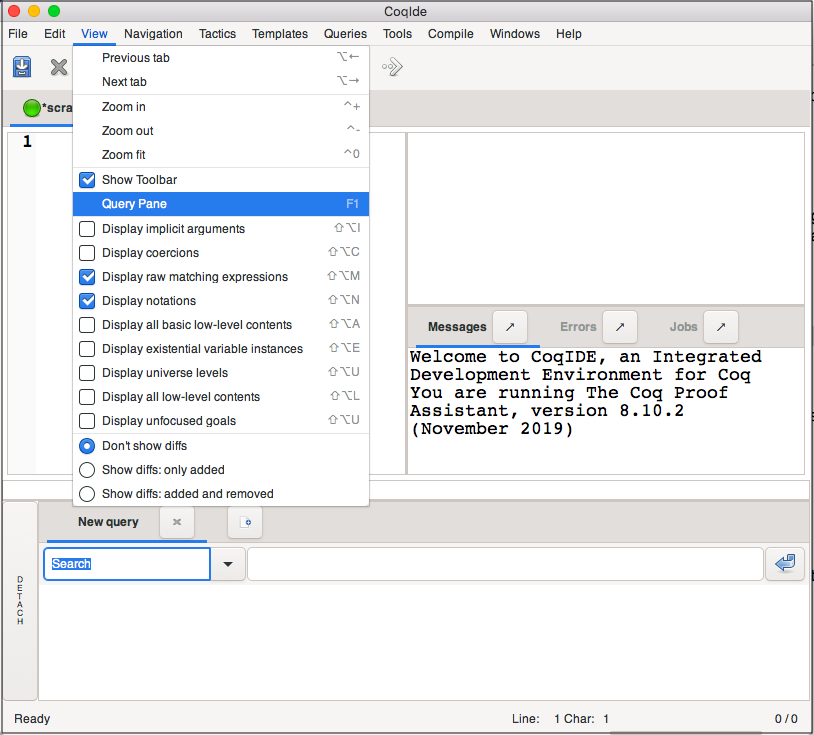
\includegraphics[width=15cm]
        {CoqScreenshots/query_pane_10.png}}
\end{minipage}

\noindent
You can detach the query pane into its own window by pressing the Detach button along the lefthand side of the query pane.
This is particularly useful when you are doing proofs and need to search to find the correct property to use 
(Coq has tons of properties defined in its libraries).




\newpage
\subsection{Search} \label{search}
Searches the environment for the given name, then displays the name and type of all objects that contains the name. 
This is useful to find out information about libraries and pre-defined theorems. 

\begin{code}
	Search plus.
\end{code}
\begin{msg}
	plus\_O\_n: forall n : nat, 0 + n = n	\\
	plus\_n\_O: forall n : nat, n = n + 0	\\
	plus\_n\_Sm: forall n m : nat, S (n + m) = n + S m	\\
	plus\_Sn\_m: forall n m : nat, S n + m = S (n + m)	\\
	mult\_n\_Sm: forall n m : nat, n * m + n = n * S m		\\
	f\_equal2\_plus: forall x1 y1 x2 y2 : nat, x1 = y1 $->$ x2 = y2 $->$ x1 + x2 = y1 + y2	\\
	nat\_rect\_plus:	\\ \-\ \quad
	  forall (n m : nat) (A : Type) (f : A $->$ A) (x : A),	\\ \-\ \quad
	  nat\_rect (fun \_ : nat $=>$ A) x (fun \_ : nat $=>$ f) (n + m) =	\\ \-\ \quad
	  nat\_rect (fun \_ : nat $=>$ A) (nat\_rect (fun \_ : nat $=>$ A) x (fun \_ : nat $=>$ f) m)	
	  \\ \-\ \qquad
	    (fun \_ : nat $=>$ f) n
\end{msg}

\noindent 
Searching multiple names obtains more specific results. 

\hspace{-1cm}
\begin{tabular}{p{8cm} p{8cm}}
\begin{code}
	Search plus 0. \\
\end{code}&
\begin{msg}
	plus\_O\_n: forall n : nat, 0 + n = n	\\
	plus\_n\_O: forall n : nat, n = n + 0
\end{msg}
\end{tabular}

\noindent 
If you haven't loaded the library corresponding to what you are searching, you will get fewer results; you may need to load the library if you can't find what you need. For example,
\begin{code}
	Search plus Nat.odd.
\end{code}
yields no results when the Arith library hasn't been added, but once we have imported the library we receive five results.
\begin{code}
	\cmd{Require Import} Arith. 	\\
	Search plus Nat.odd.
\end{code}
\begin{msg}
	Nat.odd\_add\_even: forall n m : nat, Nat.Even m $->$ Nat.odd (n + m) = Nat.odd n	\\
	Nat.odd\_add: forall n m : nat, Nat.odd (n + m) = xorb (Nat.odd n) (Nat.odd m)		\\
	Nat.odd\_add\_mul\_even: forall n m p : nat, Nat.Even m $->$ Nat.odd (n + m * p) = Nat.odd n	\\
	Nat.odd\_add\_mul\_2: forall n m : nat, Nat.odd (n + 2 * m) = Nat.odd n	\\
	Nat.div2\_odd: forall a : nat, a = 2 * Nat.div2 a + Nat.b2n (Nat.odd a)
\end{msg}

\noindent
You can also search for patterns: enclose the pattern in parentheses, and use an underscore for arbitrary terms.
\begin{code}
	Search $(\sim \_ <-> \_\ )$.
\end{code}
\begin{msg}
	neg\_false: forall A : Prop, $\sim$ A $<->$ (A $<->$ False)		\\
	not\_iff\_compat: forall A B : Prop, A $<->$ B $->$ $\sim$ A $<->$ $\sim$ B
\end{msg}




\subsection{SearchRewrite} \label{search_rewrite}
Searches the environment for a statement with an equality that contains the given pattern on at least one side.
\begin{code}
	SearchRewrite $(\_ * \_\ / \_\ )$.
\end{code}
\begin{msg}
	Nat.div\_mul: forall a b : nat, b $<>$ 0 $->$ a * b / b = a	\\
	Nat.divide\_div\_mul\_exact: 
 		forall a b c : nat, b $<>$ 0 $->$ Nat.divide b a $->$ c * a / b = c * (a / b)	\\
	Nat.div\_mul\_cancel\_l: forall a b c : nat, b $<>$ 0 $->$ c $<>$ 0 $->$ c * a / (c * b) = a / b	\\
	Nat.div\_mul\_cancel\_r: forall a b c : nat, b $<>$ 0 $->$ c $<>$ 0 $->$ a * c / (b * c) = a / b	\\
	Nat.lcm\_equiv1:
  		forall a b : nat, Nat.gcd a b $<>$ 0 $->$ a * (b / Nat.gcd a b) = a * b / Nat.gcd a b	\\
	Nat.lcm\_equiv2:
  		forall a b : nat, Nat.gcd a b $<>$ 0 $->$ a / Nat.gcd a b * b = a * b / Nat.gcd a b
\end{msg}





\subsection{Check} \label{check}
Displays the type of the given term.

\hspace{-1cm}
\begin{tabular}{p{8cm} p{8cm}}
	\begin{code} 	\cmd{Check} 0. 				\end{code}	%1
	\begin{code}	\cmd{Check} nat.				\end{code}	%2
	\begin{code}	\cmd{Check} plus.				\end{code}	%3
	&
	\begin{msg} 	0  : nat 						\end{msg}		%1
	\begin{msg}	nat : Set						\end{msg}		%2
	\begin{msg}	Nat.add : nat $->$ nat $->$ nat		\end{msg}		%3
\end{tabular}



\subsection{About} \label{about}
Displays information about the object with the given name 
(i.e. its kind, type, arguments).

\hspace{-1cm}
\begin{tabular}{p{8cm} p{8cm}}
	\begin{code} 	
		\cmd{About} plus. 	\\		
	\end{code}	
	&
	\begin{msg} 	
		Notation plus := Init.Nat.add	\\
		Expands to: Notation Coq.Init.Peano.plus
	\end{msg}
\end{tabular}





\subsection{Locate} \label{locate}
Displays the full name of the given term and what Coq module it is defined in.

\hspace{-1cm}
\begin{tabular}{p{8cm} p{8cm}}
	\begin{code} 	Locate plus. 					\end{code}	%1
	\begin{code} 	Locate nat. 					\end{code}	%2
	&
	\begin{msg} 	Notation Coq.Init.Peano.plus		\end{msg}		%1
	\begin{msg} 	Inductive Coq.Init.Datatypes.nat	\end{msg}		%2
\end{tabular}




\subsection{Print} \label{print}
Displays information about the given name.

\hspace{-1cm}
\begin{tabular}{p{8cm} p{8cm}}
	\begin{code} 	\cmd{Print} plus. 				\end{code}
	&
	\begin{msg} 	Notation plus := Init.Nat.add			\end{msg}	
\end{tabular}

\noindent
It is possible to see what is currently loaded and imported in the environment with the following:

\hspace{-1cm}
\begin{tabular}{p{8cm} p{8cm}}
	\begin{code} 	\cmd{Print} Libraries. \\ \\ \\ \\ \\ \\ \\ \\ \\ \\ \\ \\ \end{code}
	&
	\begin{msg} 	
		Loaded and imported library files: 	\\ \-\ \quad
		  Coq.Init.Notations				\\ \-\ \quad
		  Coq.Init.Logic					\\ \-\ \quad
		  Coq.Init.Logic\_Type			\\ \-\ \quad
		  Coq.Init.Datatypes				\\ \-\ \quad
		  Coq.Init.Specif				\\ \-\ \quad
		  Coq.Init.Peano				\\ \-\ \quad
		  Coq.Init.Wf					\\ \-\ \quad
		  Coq.Init.Tactics				\\ \-\ \quad
		  Coq.Init.Tauto					\\ \-\ \quad
		  Coq.Init.Prelude				\\
		Loaded and not imported library files: \\ \-\ \quad
		  Coq.Init.Nat
	\end{msg}	
\end{tabular}





\subsection{Print Assumptions} \label{print_assumptions}
Displays all assumptions depended upon by the object of the given name.

\hspace{-1cm}
\begin{tabular}{p{8cm} p{8cm}}
	\begin{code} 	\cmd{Print} Assumptions plus. 			\end{code}
	&
	\begin{msg} 	Closed under the global context		\end{msg}	
\end{tabular}







%\subsection{} \label{}







\newpage
\section{Proof Tactics}
	\label{Sec: tactics}
	
This section contains brief descriptions of some commonly used proof tactics.
For the full breakdown of all Coq tactics, please refer to the Tactic Index of the Coq documentation that can be found here:
\url{https://coq.inria.fr/distrib/current/refman/coq-tacindex.html}.


\subsection{simpl} \label{simpl}
Simplify both sides of an equation.

\noindent
Examples using this tactic: 
%\ref{count_to_n},
\ref{sum_to_n}




\subsection{reflexivity} \label{reflexivity}
Check if both sides of an equation are equal. 
Will do more simplifications that simpl; tries unfolding and expanding definitions.

\noindent
Examples using this tactic: 
\ref{sum_to_n}




\subsection{trivial} \label{trivial}
A restriction of auto that is not recursive. 
Tries simple hints, like solving trivial equalities such as x=x.

\noindent
Examples using this tactic: 
%\ref{count_to_n},
\ref{sum_to_n}



\subsection{auto} \label{auto}
First attempts to use assumption, then uses intros and generates any hypotheses to use as hints and attempt to apply.

\noindent
Examples using this tactic: 



\subsection{ring} \label{ring}
Very useful when proving over numbers.
Solves equations upon polynomial expressions of a ring structure. 
Normalizes and compares results.
Uses properties like associativity, commutativity, distributivity, and constant propagation.

\noindent
Examples using this tactic: 
\ref{sum_to_n}


\subsection{discriminate} \label{discriminate}
Proves any goal in an assumption stating two structurally different terms of an inductive set are equal. For example, S (S O) = S O.

\noindent
Examples using this tactic: 



\subsection{assumption} \label{assumption}
Looks in the local context for the hypothesis. The type must be convertible to the goal.

\noindent
Examples using this tactic: 



\subsection{intros} \label{intros}
Introduces variables from the goal into the proof environment for use.

\noindent
Examples using this tactic: 
%\ref{count_to_n}, 
\ref{sum_to_n}


\subsection{contradiction} \label{contradiction}
Attempts to find a hypothesis equivalent to:
\begin{itemize}
	\item an empty inductive type (i.e. false)
	\item the negation of a single inductive type (i.e. true, x=x)
	\item two contradictory hypotheses
\end{itemize}

\noindent
Examples using this tactic: 



\subsection{induction} \label{induction}
The object must be of an inductive type to use induction. 
This generates subgoals and an induction hypothesis.

\noindent
Examples using this tactic: 
%\ref{count_to_n}



\subsection{functional induction} \label{functional induction}
Very useful for inductive/recursive functions.
Performs case analysis and induction on the definition of a function.
To use functional induction, you need to make sure to require and load FunInd, and then define the functional induction scheme.

\begin{code}
\cmd{Require} \nm{FunInd}.	\\
\Load FunInd.
\\ \\
Functional Scheme name\_ind := 
  Induction for name Sort \ty{Prop}.
\end{code}

\noindent
Examples using this tactic: 
\ref{sum_to_n}


\subsection{destruct} \label{destruct}
Creates subgoals from a more complex goal. 
Subgoals must be proven separately.
Can be used with any inductively defined type.
Can be used nested if a generated subgoal needs to be broken up further.
Allows you to specify the names of variables to be used in proving the subgoals.

\noindent
Examples using this tactic: 



\subsection{rewrite} \label{rewrite}
A way to apply previously defined assumptions.
Can use arrows $<-$ , $->$ to give directionality for the application.
Example \ref{sum_to_n} demonstrates the use of arrows to give directionality to rewrite.

\noindent
Examples using this tactic: 
%\ref{count_to_n}, 
\ref{sum_to_n}


\subsection{apply} \label{apply}
Attempts to match the current goal against the conclusion of the given term.

\noindent
Examples using this tactic:





%\subsection{} \label{}





\newpage
\section{Examples: Proving in Coq}
	\label{Sec: proof examples}
	
%\newpage
\subsection{Days of the Week Proofs} \label{days_proofs}

Please see file ``days.v'' to follow along with this example. 

~\\
This example is fairly simple, giving some basic proofs Coq. 
Please see Example \ref{days} for the more on the definitions these proofs rely on. 

\begin{code}
\Definition \nm{next\_weekday} (d:day): day :=		\\ \-\ \quad
  \match d \with								\\ \-\ \qquad
   $\mid$ monday $=>$ tuesday					\\ \-\ \qquad
   $\mid$ tuesday $=>$ wednesday				\\ \-\ \qquad
   $\mid$ wednesday $=>$ thursday				\\ \-\ \qquad
   $\mid$ thursday $=>$ friday					\\ \-\ \qquad
   $\mid$ friday $=>$ monday					\\ \-\ \qquad
   $\mid$ saturday $=>$ monday				\\ \-\ \qquad
   $\mid$ sunday $=>$ monday					\\ \-\ \quad
  \End.
\end{code}

% PROOF 1
\noindent
We can do a simple proof to check that the results are as expected.

\hspace{-1cm}
\begin{tabular}{p{8cm} p{8cm}}
\begin{code}
	\Example \nm{test\_next\_weekday}:			\\ \-\ \quad
	  (next\_weekday (next\_weekday saturday)) 	\\ \-\ \qquad
	  	= tuesday.							\\
	\Proof.
\end{code}
&
\begin{goal}
1 subgoal			\\
\_\_\_\_\_\_\_\_\_\_\_\_\_\_\_\_\_\_\_\_\_\_\_\_\_\_\_\_\_\_\_\_\_\_\_\_\_\_(1/1)	\\
next\_weekday (next\_weekday saturday) = tuesday
\end{goal}
\end{tabular}

\noindent 
First, we can apply tactic \TT{simpl} to evaluate the uses of the \TT{next\_weekday} function: 

\hspace{-1cm}
\begin{tabular}{p{8cm} p{8cm}}
\begin{code}
simpl.
\end{code}
&
\begin{goal}
1 subgoal			\\
\_\_\_\_\_\_\_\_\_\_\_\_\_\_\_\_\_\_\_\_\_\_\_\_\_\_\_\_\_\_\_\_\_\_\_\_\_\_(1/1)	\\
tuesday = tuesday
\end{goal}
\end{tabular}

\noindent 
We can then use the tactic \TT{reflexivity} to show that \TT{tuesday} is equal to \TT{tuesday}: 

\hspace{-1cm}
\begin{tabular}{p{8cm} p{8cm}}
\begin{code}
reflexivity.
\end{code}
&
\begin{goal}
No more subgoals.
\end{goal}
\end{tabular}

\noindent 
Finally, we finish our proof with the command \TT{\Qed}:

\hspace{-1cm}
\begin{tabular}{p{8cm} p{8cm}}
\begin{code}
\Qed. 
\end{code}
&
\begin{msg}
test\_next\_weekday is defined
\end{msg}
\end{tabular}



% PROOF 2
\noindent 
We can also do a simple proof to show something will not be true, like that 
\TT{next\_weekday monday} is not \TT{friday} ($<>$ is used to say that two terms are not equal): 

\hspace{-1cm}
\begin{tabular}{p{8cm} p{8cm}}
\begin{code}
\Example \nm{next\_weekday\_monday\_friday}: \\ \-\ \quad 
  next\_weekday monday $<>$ friday. 		\\
\Proof. 
\end{code}
&
\begin{msg}
1 subgoal				\\
\_\_\_\_\_\_\_\_\_\_\_\_\_\_\_\_\_\_\_\_\_\_\_\_\_\_\_\_\_\_\_\_\_\_\_\_\_\_(1/1)	\\
next\_weekday monday $<>$ friday		
\end{msg}
\end{tabular}

\noindent 
This proof can be solved with a single tactic, \TT{discriminate}, which can be used to prove that two elements of an inductive type are different from each other: 

\hspace{-1cm}
\begin{tabular}{p{8cm} p{8cm}}
\begin{code}
discriminate. 
\end{code}
&
\begin{msg}
No more subgoals.
\end{msg}
\end{tabular}

\noindent 
Again, we finish our proof with the command \TT{\Qed}:

\hspace{-1cm}
\begin{tabular}{p{8cm} p{8cm}}
\begin{code}
\Qed. 
\end{code}
&
\begin{msg}
next\_weekday\_monday\_friday is defined
\end{msg}
\end{tabular}



% PROOF 3
\noindent
We can also prove more general things, such as that \TT{sunday} is not the next weekday for any given day \TT{d}: 

\hspace{-1cm}
\begin{tabular}{p{8cm} p{8cm}}
\begin{code}
\Example \nm{next\_weekday\_is\_not\_sunday}: 		\\
\Forall (d:day), next\_weekday d $<>$ sunday.		\\
\Proof. 
\end{code}
&
\begin{goal}
1 subgoal				\\
\_\_\_\_\_\_\_\_\_\_\_\_\_\_\_\_\_\_\_\_\_\_\_\_\_\_\_\_\_\_\_\_\_\_\_\_\_\_(1/1)	\\
\Forall d : day, next\_weekday d $<>$ sunday
\end{goal}
\end{tabular}

\noindent
Since we are using the variable \TT{d}, we need to introduce it into the proof environment: 

\hspace{-1cm}
\begin{tabular}{p{8cm} p{8cm}}
\begin{code}
intros d. 
\end{code}
&
\begin{goal}
1 subgoal				\\
d : day				\\
\_\_\_\_\_\_\_\_\_\_\_\_\_\_\_\_\_\_\_\_\_\_\_\_\_\_\_\_\_\_\_\_\_\_\_\_\_\_(1/1)	\\
next\_weekday d $<>$ sunday
\end{goal}
\end{tabular}

\noindent
Here, we can use the \TT{destruct} tactic to do case analysis over all possible days that \TT{d} can be, giving us 7 subgoals (i.e., one for each possible day of the week): 

\hspace{-1cm}
\begin{tabular}{p{8cm} p{8cm}}
\begin{code}
destruct d.
\end{code}
&
\begin{goal}		
7 subgoals													\\
\_\_\_\_\_\_\_\_\_\_\_\_\_\_\_\_\_\_\_\_\_\_\_\_\_\_\_\_\_\_\_\_\_\_\_\_\_\_(1/7)	\\
next\_weekday monday $<>$ sunday								\\
\_\_\_\_\_\_\_\_\_\_\_\_\_\_\_\_\_\_\_\_\_\_\_\_\_\_\_\_\_\_\_\_\_\_\_\_\_\_(2/7)	\\
next\_weekday tuesday $<>$ sunday								\\
\_\_\_\_\_\_\_\_\_\_\_\_\_\_\_\_\_\_\_\_\_\_\_\_\_\_\_\_\_\_\_\_\_\_\_\_\_\_(3/7)	\\
next\_weekday wednesday $<>$ sunday								\\
\_\_\_\_\_\_\_\_\_\_\_\_\_\_\_\_\_\_\_\_\_\_\_\_\_\_\_\_\_\_\_\_\_\_\_\_\_\_(4/7)	\\
next\_weekday thursday $<>$ sunday								\\	
\_\_\_\_\_\_\_\_\_\_\_\_\_\_\_\_\_\_\_\_\_\_\_\_\_\_\_\_\_\_\_\_\_\_\_\_\_\_(5/7)	\\
next\_weekday friday $<>$ sunday									\\
\_\_\_\_\_\_\_\_\_\_\_\_\_\_\_\_\_\_\_\_\_\_\_\_\_\_\_\_\_\_\_\_\_\_\_\_\_\_(6/7)	\\
next\_weekday saturday $<>$ sunday								\\
\_\_\_\_\_\_\_\_\_\_\_\_\_\_\_\_\_\_\_\_\_\_\_\_\_\_\_\_\_\_\_\_\_\_\_\_\_\_(7/7)	\\
next\_weekday sunday $<>$ sunday
\end{goal}
\end{tabular}

\noindent
We now need to go through each subgoal and prove that it is not equal. 
Like in the last proof we did, we will use the tactic \TT{discriminate} 
-- we can first apply \TT{simpl} to show the result of the given evaluation of \TT{next\_weekday}. 
For example, we enter into the first subgoal:

\hspace{-1cm}
\begin{tabular}{p{8cm} p{8cm}}
\begin{code}
- 
\end{code}
&
\begin{goal}
1 subgoal														\\
\_\_\_\_\_\_\_\_\_\_\_\_\_\_\_\_\_\_\_\_\_\_\_\_\_\_\_\_\_\_\_\_\_\_\_\_\_\_(1/1)	\\
next\_weekday monday $<>$ sunday						
\end{goal}
\end{tabular}

\noindent
Then we call \TT{simpl}:

\hspace{-1cm}
\begin{tabular}{p{8cm} p{8cm}}
\begin{code}
- simpl. 
\end{code}
&
\begin{goal}
1 subgoal														\\
\_\_\_\_\_\_\_\_\_\_\_\_\_\_\_\_\_\_\_\_\_\_\_\_\_\_\_\_\_\_\_\_\_\_\_\_\_\_(1/1)	\\
tuesday $<>$ sunday
\end{goal}
\end{tabular}

\noindent
Then we can use \TT{discriminate} to finish this subgoal:

\hspace{-1cm}
\begin{tabular}{p{8cm} p{8cm}}
\begin{code}
discriminate.
\end{code}
&
\begin{goal}
This subproof is complete, but there are some unfocused goals:	\\ 	\\
\_\_\_\_\_\_\_\_\_\_\_\_\_\_\_\_\_\_\_\_\_\_\_\_\_\_\_\_\_\_\_\_\_\_\_\_\_\_(1/6)	\\
next\_weekday tuesday $<>$ sunday								\\
\_\_\_\_\_\_\_\_\_\_\_\_\_\_\_\_\_\_\_\_\_\_\_\_\_\_\_\_\_\_\_\_\_\_\_\_\_\_(2/6)	\\
next\_weekday wednesday $<>$ sunday								\\
\_\_\_\_\_\_\_\_\_\_\_\_\_\_\_\_\_\_\_\_\_\_\_\_\_\_\_\_\_\_\_\_\_\_\_\_\_\_(3/6)	\\
next\_weekday thursday $<>$ sunday								\\	
\_\_\_\_\_\_\_\_\_\_\_\_\_\_\_\_\_\_\_\_\_\_\_\_\_\_\_\_\_\_\_\_\_\_\_\_\_\_(4/6)	\\
next\_weekday friday $<>$ sunday									\\
\_\_\_\_\_\_\_\_\_\_\_\_\_\_\_\_\_\_\_\_\_\_\_\_\_\_\_\_\_\_\_\_\_\_\_\_\_\_(5/6)	\\
next\_weekday saturday $<>$ sunday								\\
\_\_\_\_\_\_\_\_\_\_\_\_\_\_\_\_\_\_\_\_\_\_\_\_\_\_\_\_\_\_\_\_\_\_\_\_\_\_(6/6)	\\
next\_weekday sunday $<>$ sunday
\end{goal}
\end{tabular}

\noindent
The proofs for each of these subgoals can be simply solved using \TT{discriminate} 
(given they are nearly identical to the above, they are shown grouped together): 

\hspace{-1cm}
\begin{tabular}{p{8cm} p{8cm}}
\begin{code}
- discriminate.		\\
- discriminate.		\\
- discriminate.		\\
- discriminate.		\\
- discriminate.		\\
- discriminate.	
\end{code}
&
\begin{goal}
No more subgoals.
\end{goal}
\end{tabular}

\noindent
As always, we close out the completed proof using \TT{\Qed}:

\hspace{-1cm}
\begin{tabular}{p{8cm} p{8cm}}
\begin{code}
\Qed. 
\end{code}
&
\begin{msg}
next\_weekday\_is\_not\_sunday is defined
\end{msg}
\end{tabular}



% PROOF 4
\noindent
Now, you may be wondering why there isn't a simpler way to show that all cases can be solved using the same tactic. 
There is, in fact, syntax to do just that -- so we can prove the same thing regarding \TT{saturday} as we did above with \TT{sunday} using the following: 

\hspace{-1cm}
\begin{tabular}{p{8cm} p{8cm}}
\begin{code}
Example \nm{next\_weekday\_is\_not\_saturday}: 	\\
\Forall (d:day), next\_weekday d $<>$ saturday. 	\\
\Proof.
\end{code}
&
\begin{goal}
1 subgoal			\\
\_\_\_\_\_\_\_\_\_\_\_\_\_\_\_\_\_\_\_\_\_\_\_\_\_\_\_\_\_\_\_\_\_\_\_\_\_\_(1/1)	\\
\Forall d : day, next\_weekday d $<>$ saturday
\end{goal}
\end{tabular}

\noindent
We make sure to introduce the variable \TT{d} first:

\hspace{-1cm}
\begin{tabular}{p{8cm} p{8cm}}
\begin{code}
intros d.
\end{code}
&
\begin{goal}
1 subgoal			\\
d : day			\\
\_\_\_\_\_\_\_\_\_\_\_\_\_\_\_\_\_\_\_\_\_\_\_\_\_\_\_\_\_\_\_\_\_\_\_\_\_\_(1/1)	\\ 
next\_weekday d $<>$ saturday
\end{goal}
\end{tabular}

\noindent
Now, as with the previous proof, we want to use \TT{destruct} on \TT{d}, 
then apply \TT{discriminate} to all subgoals, which we can do by writing the following 
(the use of the semicolon (i.e., \TT{t1 ; t2}) tells the proof environment to apply the tactic following it (i.e., \TT{t1}) to the result of the tactic before it (i.e., \TT{t2})): 

\hspace{-1cm}
\begin{tabular}{p{8cm} p{8cm}}
\begin{code}
destruct d; discriminate.
\end{code}
&
\begin{goal}
No more subgoals.
\end{goal}
\end{tabular}

\noindent
Finally, we close out the proof environment:

\hspace{-1cm}
\begin{tabular}{p{8cm} p{8cm}}
\begin{code}
\Qed.
\end{code}
&
\begin{msg}
next\_weekday\_is\_not\_saturday is defined
\end{msg}
\end{tabular}






\newpage
\subsection{List Rev} \label{list_rev}

See Coq file ``rev\_list.v'' to follow along with this example. 


~\\
In this example, we want to prove that the reverse of the reverse of a list is the original list 
(i.e., \TT{rev (rev xs) = xs}). 
In order to do this, we must first prove a few supplementary lemmas in order to obtain 
our original goal. 
First, in order to use list notations, we must either define them, or use the command 
\TT{\Load List.}:

\hspace{-1cm}
\begin{tabular}{l}\begin{code}		\Load List.			\end{code}\end{tabular}

~\\
Then we start with defining \TT{list\_nil}, a lemma to show that a list \TT{xs} appended to 
nil (i.e., the empty list \TT{[ ]}) is \TT{xs}: 

\hspace{-1cm}
\begin{tabular}{p{8cm} p{8cm}}
\begin{code}
\Lemma \nm{list\_nil} : 			\\
\Forall (xs : Datatypes.list nat),		\\
xs ++ [ ] = xs.	
\end{code}
&
\begin{goal}
1 subgoal	\\
\_\_\_\_\_\_\_\_\_\_\_\_\_\_\_\_\_\_\_\_\_\_\_\_\_\_\_\_\_\_\_\_\_\_\_\_\_\_(1/1)	\\
\Forall xs : Datatypes.list nat, 		
xs ++ [\ ] = xs
\end{goal}
\end{tabular}

\noindent
Next, we open the proof environment using the command \TT{\Proof.}: 

\hspace{-1cm}
\begin{tabular}{p{8cm} p{8cm}}
\begin{code}
\Proof.
\end{code}
&
\begin{goal}
1 subgoal	\\
\_\_\_\_\_\_\_\_\_\_\_\_\_\_\_\_\_\_\_\_\_\_\_\_\_\_\_\_\_\_\_\_\_\_\_\_\_\_(1/1)	\\
\Forall xs : Datatypes.list nat, 		
xs ++ [\ ] = xs
\end{goal}
\end{tabular}


\noindent
Then we introduce the variable we using for our list, \TT{xs}, using \TT{intros xs.}:

\hspace{-1cm}
\begin{tabular}{p{8cm} p{8cm}}
\begin{code}
intros xs.
\end{code}
&
\begin{goal}
1 subgoal														\\
xs : Datatypes.list nat											\\
\_\_\_\_\_\_\_\_\_\_\_\_\_\_\_\_\_\_\_\_\_\_\_\_\_\_\_\_\_\_\_\_\_\_\_\_\_\_(1/1)	\\
xs ++ [\ ] = xs
\end{goal}
\end{tabular}

\noindent
Next, we can use induction on the variable \TT{xs} to leverage the inductive nature of the list type 
and split our main goal into two subgoals: 

\hspace{-1cm}
\begin{tabular}{p{8cm} p{8cm}}
\begin{code}
induction xs.
\end{code}
&
\begin{goal}
2 subgoals													\\
\_\_\_\_\_\_\_\_\_\_\_\_\_\_\_\_\_\_\_\_\_\_\_\_\_\_\_\_\_\_\_\_\_\_\_\_\_\_(1/2)	\\
$[\ ] ++ [\ ] = [\ ]$												\\
\_\_\_\_\_\_\_\_\_\_\_\_\_\_\_\_\_\_\_\_\_\_\_\_\_\_\_\_\_\_\_\_\_\_\_\_\_\_(2/2)	\\
(a :: xs) $++$ [\ ] = a :: xs
\end{goal}
\end{tabular}

\noindent
Now, we enter into the first subgoal using \TT{-}:

\hspace{-1cm}
\begin{tabular}{p{8cm} p{8cm}}
\begin{code}
- 
\end{code}
&
\begin{goal}
1 subgoal														\\
\_\_\_\_\_\_\_\_\_\_\_\_\_\_\_\_\_\_\_\_\_\_\_\_\_\_\_\_\_\_\_\_\_\_\_\_\_\_(1/1)	\\
$[\ ] ++ [\ ] = [\ ]$												\\
															\\
Unfocused Goals:												\\
\_\_\_\_\_\_\_\_\_\_\_\_\_\_\_\_\_\_\_\_\_\_\_\_\_\_\_\_\_\_\_\_\_\_\_\_\_\_		\\
(a :: xs) ++ [\ ] = a :: xs										
\end{goal}
\end{tabular}

\noindent
We can use the tactic \TT{auto} to solve this subgoal:

\hspace{-1cm}
\begin{tabular}{p{8cm} p{8cm}}
\begin{code}
- auto. 
\end{code}
&
\begin{goal}
This subproof is complete, but there are some unfocused goals:			\\
\_\_\_\_\_\_\_\_\_\_\_\_\_\_\_\_\_\_\_\_\_\_\_\_\_\_\_\_\_\_\_\_\_\_\_\_\_\_		\\
(a :: xs) ++ [\ ] = a :: xs									
\end{goal}
\end{tabular}


\noindent
Now, we enter into the second subgoal using \TT{-}:

\hspace{-1cm}
\begin{tabular}{p{8cm} p{8cm}}
\begin{code}
- 
\end{code}
&
\begin{goal}
1 subgoal														\\
a : nat														\\
xs : Datatypes.list nat											\\
IHxs : xs ++ [\ ] = xs												\\
\_\_\_\_\_\_\_\_\_\_\_\_\_\_\_\_\_\_\_\_\_\_\_\_\_\_\_\_\_\_\_\_\_\_\_\_\_\_(1/1)	\\
(a :: xs) ++ [\ ] = a :: xs	
\end{goal}
\end{tabular}

\noindent
For this subgoal, we want to be able to use the inductive hypothesis, and to do that 
we can use the tactic \TT{simpl} to remove the parentheses around \TT{a :: xs}: 

\hspace{-1cm}
\begin{tabular}{p{8cm} p{8cm}}
\begin{code}
- simpl.
\end{code}
&
\begin{goal}
1 subgoal														\\
a : nat														\\
xs : Datatypes.list nat											\\
IHxs : xs ++ [\ ] = xs												\\
\_\_\_\_\_\_\_\_\_\_\_\_\_\_\_\_\_\_\_\_\_\_\_\_\_\_\_\_\_\_\_\_\_\_\_\_\_\_(1/1)	\\
a :: xs ++ [\ ] = a :: xs	
\end{goal}
\end{tabular}

\noindent
Now we can use the tactic \TT{rewrite ->} to use the inductive hypothesis to rewrite 
\TT{xs ++ [\ ]} to \TT{xs} on the left-hand side: 

\hspace{-1cm}
\begin{tabular}{p{8cm} p{8cm}}
\begin{code}
rewrite $->$ IHxs.
\end{code}
&
\begin{goal}
1 subgoal														\\
a : nat														\\
xs : Datatypes.list nat											\\
IHxs : xs ++ [\ ] = xs												\\
\_\_\_\_\_\_\_\_\_\_\_\_\_\_\_\_\_\_\_\_\_\_\_\_\_\_\_\_\_\_\_\_\_\_\_\_\_\_(1/1)	\\
a :: xs = a :: xs	
\end{goal}
\end{tabular}

\noindent
We can then use the tactic \TT{auto} to finish this subgoal: 

\hspace{-1cm}
\begin{tabular}{p{8cm} p{8cm}}
\begin{code} 
auto. 
\end{code}
&
\begin{goal}
No more subgoals.
\end{goal}
\end{tabular}

\noindent
Finally, we finish up the proof of \TT{list\_nil} with the proof completion command, \TT{\Qed.}: 

\hspace{-1cm}
\begin{tabular}{p{8cm} p{8cm}}
\begin{code} 
\Qed. 
\end{code}
&
\begin{msg}
list\_nil is defined
\end{msg}
\end{tabular}

\noindent
Next, we need to define a lemma for list associativity, \TT{list\_assoc}:

\hspace{-1cm}
\begin{tabular}{p{7cm} p{9cm}}
\begin{code} 
\Lemma \nm{list\_assoc} : 				\\
\Forall (xs ys zs : Datatypes.list nat),			\\
(xs ++ ys) ++ zs = xs ++ (ys ++ zs).
\end{code}
&
\begin{goal}
1 subgoal														\\
\_\_\_\_\_\_\_\_\_\_\_\_\_\_\_\_\_\_\_\_\_\_\_\_\_\_\_\_\_\_\_\_\_\_\_\_\_\_(1/1)	\\
forall xs ys zs : Datatypes.list nat,									\\
(xs ++ ys) ++ zs = xs ++ ys ++ zs
\end{goal}
\end{tabular}

\noindent
Then we enter the proof environment, and introduce our local variables:

\hspace{-1cm}
\begin{tabular}{p{7cm} p{9cm}}
\begin{code} 
\Proof. 			\\
intros xs ys zs. 	
\end{code}
&
\begin{goal}
1 subgoal														\\
xs, ys, zs : Datatypes.list nat										\\
\_\_\_\_\_\_\_\_\_\_\_\_\_\_\_\_\_\_\_\_\_\_\_\_\_\_\_\_\_\_\_\_\_\_\_\_\_\_(1/1)	\\
(xs ++ ys) ++ zs = xs ++ ys ++ zs
\end{goal}
\end{tabular}

\noindent
We then specify we would like to complete the proof by using induction on list \TT{xs}:

\hspace{-1cm}
\begin{tabular}{p{7cm} p{9cm}}
\begin{code} 
induction xs.
\end{code}
&
\begin{goal}
2 subgoals
ys, zs : Datatypes.list nat											\\
\_\_\_\_\_\_\_\_\_\_\_\_\_\_\_\_\_\_\_\_\_\_\_\_\_\_\_\_\_\_\_\_\_\_\_\_\_\_(1/2)	\\
([\ ] ++ ys) ++ zs = [\ ] ++ ys ++ zs									\\
\_\_\_\_\_\_\_\_\_\_\_\_\_\_\_\_\_\_\_\_\_\_\_\_\_\_\_\_\_\_\_\_\_\_\_\_\_\_(2/2)	\\
((a :: xs) ++ ys) ++ zs = (a :: xs) ++ ys ++ zs
\end{goal}
\end{tabular}

\noindent
Then we can enter into the first subgoal, and complete the proof of this subgoal by simply 
using the tactic \TT{auto}:

\hspace{-1cm}
\begin{tabular}{p{7cm} p{9cm}}
\begin{code} 
- auto.
\end{code}
&
\begin{goal}
This subproof is complete, but there are some unfocused goals:			\\
\_\_\_\_\_\_\_\_\_\_\_\_\_\_\_\_\_\_\_\_\_\_\_\_\_\_\_\_\_\_\_\_\_\_\_\_\_\_(1/1)	\\
((a :: xs) ++ ys) ++ zs = (a :: xs) ++ ys ++ zs
\end{goal}
\end{tabular}

\noindent
Then we can enter into the second subgoal, and view our inductive hypothesis:

\hspace{-1cm}
\begin{tabular}{p{7cm} p{9cm}}
\begin{code} 
- 
\end{code}
&
\begin{goal}
1 subgoal														\\
a : nat														\\
xs, ys, zs : Datatypes.list nat										\\
IHxs : (xs ++ ys) ++ zs =   xs ++ ys ++ zs								\\
\_\_\_\_\_\_\_\_\_\_\_\_\_\_\_\_\_\_\_\_\_\_\_\_\_\_\_\_\_\_\_\_\_\_\_\_\_\_(1/1)	\\
((a :: xs) ++ ys) ++ zs = (a :: xs) ++ ys ++ zs
\end{goal}
\end{tabular}

\noindent
We can use the tactic \TT{simpl} to simplify our subgoal, removing some of the layers of parentheses:

\hspace{-1cm}
\begin{tabular}{p{7cm} p{9cm}}
\begin{code} 
- simpl.
\end{code}
&
\begin{goal}
1 subgoal														\\
a : nat														\\
xs, ys, zs : Datatypes.list nat										\\
IHxs : (xs ++ ys) ++ zs =   xs ++ ys ++ zs								\\
\_\_\_\_\_\_\_\_\_\_\_\_\_\_\_\_\_\_\_\_\_\_\_\_\_\_\_\_\_\_\_\_\_\_\_\_\_\_(1/1)	\\
a :: (xs ++ ys) ++ zs = a :: xs ++ ys ++ zs
\end{goal}
\end{tabular}

\noindent
Now we can use the \TT{rewrite} tactic to further our proof by using the inductive hypothesis. 
As you can see above, in the right-hand side of our subgoal, 
we have the term sequence matching that of the right-hand side of the inductive hypothesis, 
and likewise with on left-hand sides of the subgoal and inductive hypothesis. 
In the last proof, we used \TT{->}, so this time we will use \TT{<-} with \TT{rewrite} to 
illustrate the difference:

\hspace{-1cm}
\begin{tabular}{p{7cm} p{9cm}}
\begin{code} 
rewrite $<-$ IHxs.
\end{code}
&
\begin{goal}
1 subgoal														\\
a : nat														\\
xs, ys, zs : Datatypes.list nat										\\
IHxs : (xs ++ ys) ++ zs = xs ++ ys ++ zs								\\
\_\_\_\_\_\_\_\_\_\_\_\_\_\_\_\_\_\_\_\_\_\_\_\_\_\_\_\_\_\_\_\_\_\_\_\_\_\_(1/1)	\\
a :: (xs ++ ys) ++ zs = a :: (xs ++ ys) ++ zs
\end{goal}
\end{tabular}

\noindent
Now we are left with identical left- and right-hand sides of the subgoal. 
From here, we can finish the proof of this subgoal using the tactic \TT{auto}:

\hspace{-1cm}
\begin{tabular}{p{7cm} p{9cm}}
\begin{code} 
auto.
\end{code}
&
\begin{goal}
No more subgoals.
\end{goal}
\end{tabular}

\noindent
Finally, we finish up the proof of \TT{list\_assoc} with the proof completion command, \TT{\Qed.}: 

\hspace{-1cm}
\begin{tabular}{p{7cm} p{9cm}}
\begin{code} 
\Qed. 
\end{code}
&
\begin{msg}
list\_assoc is defined
\end{msg}
\end{tabular}

\noindent
We now progress on to the lemma (\TT{rev\_list}) for proving that the reverse of two lists appended together 
(i.e., \TT{xs} appended to \TT{ys}) is equivalent to the reverse of the second list (\TT{ys}) 
appended to the reverse of the first list (\TT{xs}).

\hspace{-1cm}
\begin{tabular}{p{7cm} p{9cm}}
\begin{code} 
\Lemma \nm{rev\_list} : 				\\
\Forall (xs ys : Datatypes.list nat),		\\
rev (xs ++ ys) = (rev ys) ++ (rev xs).
\end{code}
&
\begin{goal}
1 subgoal														\\
\_\_\_\_\_\_\_\_\_\_\_\_\_\_\_\_\_\_\_\_\_\_\_\_\_\_\_\_\_\_\_\_\_\_\_\_\_\_(1/1)	\\
forall xs ys : Datatypes.list nat,										\\
rev (xs ++ ys) = rev ys ++ rev xs					
\end{goal}
\end{tabular}

\noindent
As before, we enter the proof environment, and introduce our local variables:

\hspace{-1cm}
\begin{tabular}{p{7cm} p{9cm}}
\begin{code} 
\Proof. 			\\
intros xs ys. 	
\end{code}
&
\begin{goal}
1 subgoal														\\
xs, ys : Datatypes.list nat											\\
\_\_\_\_\_\_\_\_\_\_\_\_\_\_\_\_\_\_\_\_\_\_\_\_\_\_\_\_\_\_\_\_\_\_\_\_\_\_(1/1)	\\
rev (xs ++ ys) = rev ys ++ rev xs
\end{goal}
\end{tabular}

\noindent
Then we declare we want to solve the proof by induction over \TT{xs}:

\hspace{-1cm}
\begin{tabular}{p{7cm} p{9cm}}
\begin{code} 
induction xs. 	
\end{code}
&
\begin{goal}
2 subgoals													\\
ys : Datatypes.list nat											\\
\_\_\_\_\_\_\_\_\_\_\_\_\_\_\_\_\_\_\_\_\_\_\_\_\_\_\_\_\_\_\_\_\_\_\_\_\_\_(1/2)	\\
rev ([\ ] ++ ys) = rev ys ++ rev [\ ]									\\
\_\_\_\_\_\_\_\_\_\_\_\_\_\_\_\_\_\_\_\_\_\_\_\_\_\_\_\_\_\_\_\_\_\_\_\_\_\_(2/2)	\\
rev ((a :: xs) ++ ys) = rev ys ++ rev (a :: xs)
\end{goal}
\end{tabular}

\noindent
Next, we enter into the first subgoal, an we can use \TT{simpl} to simplify the subgoal:

\hspace{-1cm}
\begin{tabular}{p{7cm} p{9cm}}
\begin{code} 
- simpl. 	
\end{code}
&
\begin{goal}
1 subgoal														\\
ys : Datatypes.list nat											\\
\_\_\_\_\_\_\_\_\_\_\_\_\_\_\_\_\_\_\_\_\_\_\_\_\_\_\_\_\_\_\_\_\_\_\_\_\_\_(1/1)	\\
rev ys = rev ys ++ [\ ]												\\
															\\
Unfocused Goals:												\\
\_\_\_\_\_\_\_\_\_\_\_\_\_\_\_\_\_\_\_\_\_\_\_\_\_\_\_\_\_\_\_\_\_\_\_\_\_\_		\\
rev ((a :: xs) ++ ys) = rev ys ++ rev (a :: xs)
\end{goal}
\end{tabular}

\noindent
We are now able to use the \TT{rewrite} tactic with our first lemma \TT{list\_nil} to further the proof:

\hspace{-1cm}
\begin{tabular}{p{7cm} p{9cm}}
\begin{code} 
rewrite $->$ list\_nil. 	
\end{code}
&
\begin{goal}
1 subgoal														\\
ys : Datatypes.list nat											\\
\_\_\_\_\_\_\_\_\_\_\_\_\_\_\_\_\_\_\_\_\_\_\_\_\_\_\_\_\_\_\_\_\_\_\_\_\_\_(1/1)	\\
rev ys = rev ys 													\\
															\\
Unfocused Goals:												\\
\_\_\_\_\_\_\_\_\_\_\_\_\_\_\_\_\_\_\_\_\_\_\_\_\_\_\_\_\_\_\_\_\_\_\_\_\_\_		\\
rev ((a :: xs) ++ ys) = rev ys ++ rev (a :: xs)
\end{goal}
\end{tabular}

\noindent
Since both sides of our subgoal equation are equal, we can use the tactic \TT{reflexivity} 
to complete this subgoal:

\hspace{-1cm}
\begin{tabular}{p{7cm} p{9cm}}
\begin{code} 
reflexivity. 	
\end{code}
&
\begin{goal}
This subproof is complete, but there are some unfocused goals:			\\
\_\_\_\_\_\_\_\_\_\_\_\_\_\_\_\_\_\_\_\_\_\_\_\_\_\_\_\_\_\_\_\_\_\_\_\_\_\_(1/1)	\\
rev ((a :: xs) ++ ys) = rev ys ++ rev (a :: xs)
\end{goal}
\end{tabular}

\noindent
We then enter the second subgoal, and attempt to use the tactic \TT{simpl} to 
obtain a set of terms in the subgoal that will match the inductive hypothesis: 

\hspace{-1cm}
\begin{tabular}{p{7cm} p{9cm}}
\begin{code} 
- simpl. 	
\end{code}
&
\begin{goal}
1 subgoal														\\
a : nat														\\
xs, ys : Datatypes.list nat											\\
IHxs : rev (xs ++ ys) =  rev ys ++ rev xs								\\
\_\_\_\_\_\_\_\_\_\_\_\_\_\_\_\_\_\_\_\_\_\_\_\_\_\_\_\_\_\_\_\_\_\_\_\_\_\_(1/1)	\\
rev (xs ++ ys) ++ [a] = rev ys ++ rev xs ++ [a]
\end{goal}
\end{tabular}

\noindent
The use of tactic \TT{simpl} succeeded in obtaining \TT{rev (xs ++ ys)} as a subset 
of the terms on the left-hand side of the equation, so we can now use the tactic 
\TT{rewrite} with the inductive hypothesis to convert this subset of terms to 
\TT{ev ys ++ rev xs}: 

\hspace{-1cm}
\begin{tabular}{p{6.5cm} p{9.5cm}}
\begin{code} 
rewrite $->$ IHxs. 	
\end{code}
&
\begin{goal}
1 subgoal														\\
a : nat														\\
xs, ys : Datatypes.list nat											\\
IHxs : rev (xs ++ ys) =  rev ys ++ rev xs								\\
\_\_\_\_\_\_\_\_\_\_\_\_\_\_\_\_\_\_\_\_\_\_\_\_\_\_\_\_\_\_\_\_\_\_\_\_\_\_(1/1)	\\
(rev ys ++ rev xs) ++ [a] = rev ys ++ rev xs ++ [a]
\end{goal}
\end{tabular}

\noindent 
We can now use the tactic \TT{apply} to apply the \TT{list\_assoc} lemma we defined 
previously on our currently subgoal: 

\hspace{-1cm}
\begin{tabular}{p{6.5cm} p{9.5cm}}
\begin{code} 
apply list\_assoc. 	
\end{code}
&
\begin{goal}
No more subgoals.
\end{goal}
\end{tabular}

\noindent
Since we have proved both of our subgoals, we can now close out the proof with 
the command \TT{\Qed.}:

\hspace{-1cm}
\begin{tabular}{p{7cm} p{9cm}}
\begin{code} 
\Qed. 	
\end{code}
&
\begin{msg}
rev\_list is defined
\end{msg}
\end{tabular}

\noindent
Finally, we can come back to our main lemma that the reverse of the reverse of a list 
is itself, \TT{rev\_rev}: 

\hspace{-1cm}
\begin{tabular}{p{7cm} p{9cm}}
\begin{code} 
\Lemma \nm{rev\_rev} : 			\\
\Forall (xs : Datatypes.list nat),	\\
rev (rev xs) = xs.		
\end{code}
&
\begin{goal}
1 subgoal														\\
\_\_\_\_\_\_\_\_\_\_\_\_\_\_\_\_\_\_\_\_\_\_\_\_\_\_\_\_\_\_\_\_\_\_\_\_\_\_(1/1)	\\
\Forall xs : Datatypes.list nat,										\\
rev (rev xs) = xs
\end{goal}
\end{tabular}

\noindent
As before, we enter the proof environment, and introduce our local variable:

\hspace{-1cm}
\begin{tabular}{p{7cm} p{9cm}}
\begin{code} 
\Proof. 			\\
intros xs. 	
\end{code}
&
\begin{goal}
1 subgoal														\\
xs : Datatypes.list nat											\\
\_\_\_\_\_\_\_\_\_\_\_\_\_\_\_\_\_\_\_\_\_\_\_\_\_\_\_\_\_\_\_\_\_\_\_\_\_\_(1/1)	\\
rev (rev xs) = xs
\end{goal}
\end{tabular}

\noindent
Here we will again use induction on list \TT{xs}:

\hspace{-1cm}
\begin{tabular}{p{7cm} p{9cm}}
\begin{code} 
induction xs. 
\end{code}
&
\begin{goal}
2 subgoals													\\
\_\_\_\_\_\_\_\_\_\_\_\_\_\_\_\_\_\_\_\_\_\_\_\_\_\_\_\_\_\_\_\_\_\_\_\_\_\_(1/2)	\\
rev (rev [\ ]) = [\ ]												\\
\_\_\_\_\_\_\_\_\_\_\_\_\_\_\_\_\_\_\_\_\_\_\_\_\_\_\_\_\_\_\_\_\_\_\_\_\_\_(2/2)	\\
rev (rev (a :: xs)) = a :: xs
\end{goal}
\end{tabular}

\noindent
We enter the first subgoal, and attempt to use the tactic \TT{auto} to complete the proof:

\hspace{-1cm}
\begin{tabular}{p{7cm} p{9cm}}
\begin{code} 
- auto. 
\end{code}
&
\begin{goal}
This subproof is complete, but there are some unfocused goals:			\\
\_\_\_\_\_\_\_\_\_\_\_\_\_\_\_\_\_\_\_\_\_\_\_\_\_\_\_\_\_\_\_\_\_\_\_\_\_\_(1/1)	\\
rev (rev (a :: xs)) = a :: xs
\end{goal}
\end{tabular}

\noindent
Since \TT{auto} has completed this subgoal, we now move to the second subgoal. 
We first use the tactic \TT{simpl} to try to obtain either the inductive hypothesis, 
or a subset of terms as in one of the lemmas we have previously defined: 

\hspace{-1cm}
\begin{tabular}{p{7cm} p{9cm}}
\begin{code} 
- simpl. 
\end{code}
&
\begin{goal}
1 subgoal														\\
a : nat														\\
xs : Datatypes.list nat											\\
IHxs : rev (rev xs) = xs											\\
\_\_\_\_\_\_\_\_\_\_\_\_\_\_\_\_\_\_\_\_\_\_\_\_\_\_\_\_\_\_\_\_\_\_\_\_\_\_(1/1)	\\
rev (rev xs ++ [a]) = a :: xs
\end{goal}
\end{tabular}

\noindent
This has left us at a point where we have the reverse of two lists appended to 
each other (i.e., \TT{rev xs} and \TT{[a]}), so we can now use the tactic 
\TT{rewrite} with out previous lemma \TT{rev\_list}:  

\hspace{-1cm}
\begin{tabular}{p{7cm} p{9cm}}
\begin{code} 
rewrite $->$ rev\_list. 
\end{code}
&
\begin{goal}
1 subgoal														\\
a : nat														\\
xs : Datatypes.list nat											\\
IHxs : rev (rev xs) = xs											\\
\_\_\_\_\_\_\_\_\_\_\_\_\_\_\_\_\_\_\_\_\_\_\_\_\_\_\_\_\_\_\_\_\_\_\_\_\_\_(1/1)	\\
rev [a] ++ rev (rev xs) = a :: xs
\end{goal}
\end{tabular}

\noindent
Now we can see that we have the left-hand side of the inductive hypothesis as 
sub-terms in the left-hand side of the subgoal, so we can now use the tactic 
\TT{rewrite} with the inductive hypothesis: 

\hspace{-1cm}
\begin{tabular}{p{7cm} p{9cm}}
\begin{code} 
rewrite $->$ IHxs. 
\end{code}
&
\begin{goal}
1 subgoal														\\
a : nat														\\
xs : Datatypes.list nat											\\
IHxs : rev (rev xs) = xs											\\
\_\_\_\_\_\_\_\_\_\_\_\_\_\_\_\_\_\_\_\_\_\_\_\_\_\_\_\_\_\_\_\_\_\_\_\_\_\_(1/1)	\\
rev [a] ++ xs = a :: xs
\end{goal}
\end{tabular}

\noindent
We will now attempt to complete the proof of this subgoal using the tactic \TT{auto}: 

\hspace{-1cm}
\begin{tabular}{p{7cm} p{9cm}}
\begin{code} 
auto. 
\end{code}
&
\begin{goal}
No more subgoals.
\end{goal}
\end{tabular}

\noindent 
Since this has succeeded in proving our final subgoal, we can now finish our proof:

\hspace{-1cm}
\begin{tabular}{p{7cm} p{9cm}}
\begin{code} 
\Qed. 
\end{code}
&
\begin{msg}
rev\_rev is defined
\end{msg}
\end{tabular}






%\newpage
%\subsection{Count to n} \label{count_to_n}
%
A simple example defining a function that takes a number n and counts to n.
We then work through proving that count n = n.

\begin{code}
	\cmd{Require Import} \nm{Arith}.		\\
	\\
	\Fixpoint \nm{count} (n : nat) : nat := 		\\ \-\ \quad
	    	\match n \with					\\ \-\ \qquad
		$\mid$ O $=>$ 0 				\\ \-\ \qquad
		$\mid$ S p $=>$ 1 + count p		\\ \-\ \quad 
		\End.
	\\ \\
	Compute count 10.
\end{code}

\noindent
Now, we can state our theorem, and begin our proof. We will see that we are initially given one subgoal as follows:

\hspace{-1cm}
\begin{tabular}{p{8cm} p{8cm}}
\begin{code}
	\Theorem \nm{count\_to\_n} : 			\\ \-\ \quad
		\Forall n:nat, count n = n.			\\
	\Proof.
\end{code}
& 
\begin{goal}
1 subgoal	\\
\_\_\_\_\_\_\_\_\_\_\_\_\_\_\_\_\_\_\_\_\_\_\_\_\_\_\_\_\_\_\_\_\_\_\_\_\_\_(1/1)	\\
forall n : nat, count n = n
\end{goal}
\end{tabular}

\noindent
Then we need to introduce the variable n into the proof environment:

\hspace{-1cm}
\begin{tabular}{p{8cm} p{8cm}}
\begin{code}
	\Proof.							\\
	intros n.
\end{code}
& 
\begin{goal}
1 subgoal	\\
n : nat	\\
\_\_\_\_\_\_\_\_\_\_\_\_\_\_\_\_\_\_\_\_\_\_\_\_\_\_\_\_\_\_\_\_\_\_\_\_\_\_(1/1)	\\
count n = n
\end{goal}
\end{tabular}

\noindent
We will use induction to split this goal into two subgoals because nat numbers are inductively defined:

\hspace{-1cm}
\begin{tabular}{p{8cm} p{8cm}}
\begin{code}
	\Proof.							\\
	intros n.							\\
	induction n \as [$\mid$ n$'$ IHn$'$].
\end{code}
& 
\begin{goal}
2 subgoals	\\	
\_\_\_\_\_\_\_\_\_\_\_\_\_\_\_\_\_\_\_\_\_\_\_\_\_\_\_\_\_\_\_\_\_\_\_\_\_\_(1/2)	\\
count 0 = 0	\\
\_\_\_\_\_\_\_\_\_\_\_\_\_\_\_\_\_\_\_\_\_\_\_\_\_\_\_\_\_\_\_\_\_\_\_\_\_\_(2/2)	\\
count (S n$'$) = S n$'$
\end{goal}
\end{tabular}

\noindent
Then we enter into a subgoal environment, and see that it focuses on the 1st subgoal:

\hspace{-1cm}
\begin{tabular}{p{8cm} p{8cm}}
\begin{code}
	\Proof.							\\
	intros n.							\\
	induction n \as [$\mid$ n$'$ IHn$'$].		\\
	\cmd{\{ -} 
\end{code}
& 
\begin{goal}
1 subgoal	\\	
\_\_\_\_\_\_\_\_\_\_\_\_\_\_\_\_\_\_\_\_\_\_\_\_\_\_\_\_\_\_\_\_\_\_\_\_\_\_(1/1)	\\
count 0 = 0	
\end{goal}
\end{tabular}

\noindent
This result is trivial to solve, and we can use the proof tactic trivial:

\hspace{-1cm}
\begin{tabular}{p{8cm} p{8cm}}
\begin{code}
	\Proof.							\\
	intros n.							\\
	induction n \as [$\mid$ n$'$ IHn$'$].		\\
	\cmd{\{ -} trivial.
\end{code}
& 
\begin{goal}
This subproof is complete, but there are some unfocused goals:	\\
\_\_\_\_\_\_\_\_\_\_\_\_\_\_\_\_\_\_\_\_\_\_\_\_\_\_\_\_\_\_\_\_\_\_\_\_\_\_(1/1)	\\
count (S n$'$) = S n$'$	
\end{goal}
\end{tabular}

\newpage
\noindent
Now we close out this subgoal and move to the next involving the induction hypothesis:

\hspace{-1cm}
\begin{tabular}{p{8cm} p{8cm}}
\begin{code}
	\Proof.							\\
	intros n.							\\
	induction n \as [$\mid$ n$'$ IHn$'$].		\\
	\cmd{\{ -} trivial. \cmd\}				\\
	\cmd{\{ -}
\end{code}
& 
\begin{goal}
1 subgoal			\\
n$'$ : nat			\\
IHn$'$ : count n$'$ = n$'$	\\
\_\_\_\_\_\_\_\_\_\_\_\_\_\_\_\_\_\_\_\_\_\_\_\_\_\_\_\_\_\_\_\_\_\_\_\_\_\_(1/1)	\\
count (S n$'$) = S n$'$	
\end{goal}
\end{tabular}

\noindent
Our first goal here is to obtain what is on the left-hand side of the induction hypothesis equation within our subgoal. we can do this using the proof tactic simpl:

\hspace{-1cm}
\begin{tabular}{p{8cm} p{8cm}}
\begin{code}
	\Proof.							\\
	intros n.							\\
	induction n \as [$\mid$ n$'$ IHn$'$].		\\
	\cmd{\{ -} trivial. \cmd\}				\\
	\cmd{\{ -} simpl.
\end{code}
& 
\begin{goal}
1 subgoal			\\
n$'$ : nat			\\
IHn$'$ : count n$'$ = n$'$	\\
\_\_\_\_\_\_\_\_\_\_\_\_\_\_\_\_\_\_\_\_\_\_\_\_\_\_\_\_\_\_\_\_\_\_\_\_\_\_(1/1)	\\
S (count n$'$) = S n$'$	
\end{goal}
\end{tabular}

\noindent
Now we are able to use the rewrite proof tactic to rewrite our goal using the induction hypothesis:

\hspace{-1cm}
\begin{tabular}{p{8cm} p{8cm}}
\begin{code}
	\Proof.							\\
	intros n.							\\
	induction n \as [$\mid$ n$'$ IHn$'$].		\\
	\cmd{\{ -} trivial. \cmd\}				\\
	\cmd{\{ -} simpl. rewrite IHn'.
\end{code}
& 
\begin{goal}
1 subgoal			\\
n$'$ : nat			\\
IHn$'$ : count n$'$ = n$'$	\\
\_\_\_\_\_\_\_\_\_\_\_\_\_\_\_\_\_\_\_\_\_\_\_\_\_\_\_\_\_\_\_\_\_\_\_\_\_\_(1/1)	\\
S n$'$ = S n$'$	
\end{goal}
\end{tabular}

\noindent 
As you can see, both sides of our goal are equal, and we can use trivial again to finish off this goal, and Coq will then tell us we have no more subgoals:

\hspace{-1cm}
\begin{tabular}{p{8cm} p{8cm}}
\begin{code}
	\Proof.							\\
	intros n.							\\
	induction n \as [$\mid$ n$'$ IHn$'$].		\\
	\cmd{\{ -} trivial. \cmd\}				\\
	\cmd{\{ -} simpl. rewrite IHn'. trivial.
\end{code}
& 
\begin{goal}
No more subgoals.
\end{goal}
\end{tabular}

\noindent
Then we can close out this proof and see that it is now defined in the environment:

\hspace{-1cm}
\begin{tabular}{p{8cm} p{8cm}}
\begin{code}
	\Theorem \nm{count\_to\_n} : 			\\ \-\ \quad
		\Forall n:nat, count n = n.			\\
	\Proof.							\\
	intros n.							\\
	induction n \as [$\mid$ n$'$ IHn$'$].			\\
	\cmd{\{ -} trivial. \cmd\}					\\
	\cmd{\{ -} simpl. rewrite IHn$'$. trivial. \cmd\}		\\
	\Qed.
\end{code}
& 
\begin{msg}
count\_to\_n is defined
\end{msg}
\end{tabular}










\newpage
\subsection{Sum to n} \label{sum_to_n}

Please see file ``sum\_1\_to\_n.v'' to follow along with this example. 

~\\
This example defines a recursive function that takes a number n and returns the sum of the numbers from one to n (i.e., \TT{$\Sigma_{i = 0}^n\ i$}).
It then proves that for all nat numbers, 2 * sum n = (1 + n) * n.
This assertion is equivalent to sum n = ((1 + n) * n) / 2; 
however, it is much easier to prove when we do not involve division.
First, a longer proof using properties of addition and multiplication will be shown, 
then the shorter version that applies the ring tactic to take care of the application of many of these properties for us.

\begin{code}
	\Load \nm{Arith}.
	\\ \\
	\Fixpoint \nm{sum} (n : nat) : nat := 		\\ \-\ \quad
	\match n \with						\\ \-\ \quad
	$\mid$ O $=>$ 0					\\ \-\ \quad
	$\mid$ S p $=>$ (S p) + (sum p)		\\ \-\ \quad
	\End.
\end{code}

\noindent
In this example, we will use functional induction to help us successfully complete our proof over the recursive function sum.
To do this, we must first make sure to require and load \TT{FunInd}, and then define the functional induction scheme.

\begin{code}
	\cmd{Require} \nm{FunInd}.	\\
	\Load FunInd.				\\
	Functional Scheme sum\_ind := Induction for sum Sort \ty{Prop}.
\end{code}

\noindent 
Next, we will define the theorem we would like to prove. 
For this function, we want to prove that $sum\ n = \frac{(1 + n) * n}{2}$; 
however, given that division is difficult to manage when proving theorems, we will rewrite this as $2 * sum\ n = (1 + n) * n$. 

\hspace{-1cm}
\begin{tabular}{p{8cm} p{8cm}}
\begin{code}
\Theorem \nm{Thm\_sum} :	\\ \-\ \quad
\Forall n:nat,				
2 * sum n = (1 + n) * n.		\\
\Proof. 
\end{code}
&
\begin{goal}
1 subgoal															\\
\_\_\_\_\_\_\_\_\_\_\_\_\_\_\_\_\_\_\_\_\_\_\_\_\_\_\_\_\_\_\_\_\_\_\_\_\_\_(1/1)		\\
\Forall n : nat, 2 * sum n = (1 + n) * n
\end{goal}
\end{tabular}



\noindent 
As usual, we need to introduce our variable\TT{n} first:

\hspace{-1cm}
\begin{tabular}{p{8cm} p{8cm}}
\begin{code}
intros n. 
\end{code}
&
\begin{goal}
1 subgoal														\\
n : nat														\\
\_\_\_\_\_\_\_\_\_\_\_\_\_\_\_\_\_\_\_\_\_\_\_\_\_\_\_\_\_\_\_\_\_\_\_\_\_\_(1/1)	\\
2 * sum n = (1 + n) * n
\end{goal}
\end{tabular}



\noindent 
Then we can declare that we would like to use functional induction to complete this proof: 

\hspace{-1cm}
\begin{tabular}{p{8cm} p{8cm}}
\begin{code}
functional induction (sum n)	\\ \-\ \quad
  using sum\_ind.
\end{code}
&
\begin{goal}
2 subgoals													\\
\_\_\_\_\_\_\_\_\_\_\_\_\_\_\_\_\_\_\_\_\_\_\_\_\_\_\_\_\_\_\_\_\_\_\_\_\_\_(1/2)	\\
2 * 0 = (1 + 0) * 0												\\
\_\_\_\_\_\_\_\_\_\_\_\_\_\_\_\_\_\_\_\_\_\_\_\_\_\_\_\_\_\_\_\_\_\_\_\_\_\_(2/2)	\\
2 * (S p + sum p) = (1 + S p) * S p
\end{goal}
\end{tabular}



\noindent 
We enter into the first subgoal: 

\hspace{-1cm}
\begin{tabular}{p{8cm} p{8cm}}
\begin{code}
- 
\end{code}
&
\begin{goal}
1 subgoal														\\
\_\_\_\_\_\_\_\_\_\_\_\_\_\_\_\_\_\_\_\_\_\_\_\_\_\_\_\_\_\_\_\_\_\_\_\_\_\_(1/1)	\\
2 * 0 = (1 + 0) * 0
\end{goal}
\end{tabular}



\noindent 
This subgoal can be solved simply by using the tactic \TT{trivial} (this tactic will recognize that both sides will evaluate to 0):

\hspace{-1cm}
\begin{tabular}{p{8cm} p{8cm}}
\begin{code}
- trivial. 
\end{code}
&
\begin{goal}
This subproof is complete, but there are some unfocused goals:			\\
\_\_\_\_\_\_\_\_\_\_\_\_\_\_\_\_\_\_\_\_\_\_\_\_\_\_\_\_\_\_\_\_\_\_\_\_\_\_(1/1) 	\\
2 * (S p + sum p) = (1 + S p) * S p
\end{goal}
\end{tabular}



\noindent 
Now we enter into our second subgoal:

\hspace{-1cm}
\begin{tabular}{p{8cm} p{8cm}}
\begin{code}
-
\end{code}
&
\begin{goal}
1 subgoal														\\
p : nat														\\
IHn0 : 2 * sum p = (1 + p) * p										\\
\_\_\_\_\_\_\_\_\_\_\_\_\_\_\_\_\_\_\_\_\_\_\_\_\_\_\_\_\_\_\_\_\_\_\_\_\_\_(1/1)	\\
2 * (S p + sum p) = (1 + S p) * S p
\end{goal}
\end{tabular}



\noindent 
Now, we need to look at our goal and decide what to do from here 
(keep in mind that we want to be able to match some part of our goal with one of the 
	sides of the equation of the inductive hypothesis).
We can try the tactic \TT{auto}, but nothing happens. 
We can try the tactic \TT{simpl}: 

\hspace{-1cm}
\begin{tabular}{p{8cm} p{8cm}}
\begin{code}
- simpl. 
\end{code}
&
\begin{goal}
1 subgoal														\\
p : nat														\\
IHn0 : 2 * sum p = (1 + p) * p										\\
\_\_\_\_\_\_\_\_\_\_\_\_\_\_\_\_\_\_\_\_\_\_\_\_\_\_\_\_\_\_\_\_\_\_\_\_\_\_(1/1)	\\
S (p + sum p + S (p + sum p + 0)) =									\\
S (p + S (p + p * S p))
\end{goal}
\end{tabular}



\noindent 
\TT{simpl} lead to the multiplications broken down, but now there are more terms to try to reason about what we should do next, so lets go back a step again. 
To get ideas on what we could apply, we can use the command \TT{Search}, such as in \TT{Search Nat.add.}
We can see that it is possible to apply \TT{Nat.add\_succ\_comm} to the right hand side of our goal:


\hspace{-1cm}
\begin{tabular}{p{8cm} p{8cm}}
\begin{code}
rewrite $<-$ Nat.add\_succ\_comm.
\end{code}
&
\begin{goal}
1 subgoal														\\
p : nat														\\
IHn0 : 2 * sum p = (1 + p) * p										\\
\_\_\_\_\_\_\_\_\_\_\_\_\_\_\_\_\_\_\_\_\_\_\_\_\_\_\_\_\_\_\_\_\_\_\_\_\_\_(1/1)	\\
2 * (S p + sum p) = (2 + p) * S p
\end{goal}
\end{tabular}



\noindent 
This doesn't make the goal more complex, but it also doesn't particularly help us get closer to being able to use the inductive hypothesis to make substitutions in our goal. 
We can use \TT{Search Nat.mul.} to try to give us some more ideas of properties we could use to get to that point. 
When looking through the results, \TT{Nat.mul\_add\_distr\_r} and \TT{Nat.mul\_add\_distr\_l} stood out to me as being helpful, so we can try those next:

\hspace{-1cm}
\begin{tabular}{p{8cm} p{8cm}}
\begin{code}
rewrite $->$ Nat.mul\_add\_distr\_r.
\end{code}
&
\begin{goal}
1 subgoal														\\
p : nat														\\
IHn0 : 2 * sum p = (1 + p) * p										\\
\_\_\_\_\_\_\_\_\_\_\_\_\_\_\_\_\_\_\_\_\_\_\_\_\_\_\_\_\_\_\_\_\_\_\_\_\_\_(1/1)	\\
2 * (S p + sum p) = 2 * S p + p * S p
\end{goal}
\end{tabular}



\noindent 
This helped us get rid of the parentheses on the right hand side of the goal, but didn't really get us closer to substituting in the inductive hypothesis. 
Lets try \TT{Nat.mul\_add\_distr\_l} next: 

\hspace{-1cm}
\begin{tabular}{p{8cm} p{8cm}}
\begin{code}
rewrite $->$ Nat.mul\_add\_distr\_l.
\end{code}
&
\begin{goal}
1 subgoal														\\
p : nat														\\
IHn0 : 2 * sum p = (1 + p) * p										\\
\_\_\_\_\_\_\_\_\_\_\_\_\_\_\_\_\_\_\_\_\_\_\_\_\_\_\_\_\_\_\_\_\_\_\_\_\_\_(1/1)	\\
2 * S p + 2 * sum p = 2 * S p + p * S p
\end{goal}
\end{tabular}



\noindent 
Now we have the left hand side of the inductive hypothesis, \TT{2 * sum p}, in our goal, so we can use the tactic \TT{rewrite} with the inductive hypothesis \TT{IHn0}: 

\hspace{-1cm}
\begin{tabular}{p{8cm} p{8cm}}
\begin{code}
rewrite $->$ IHn0.
\end{code}
&
\begin{goal}
1 subgoal														\\
p : nat														\\
IHn0 : 2 * sum p = (1 + p) * p										\\
\_\_\_\_\_\_\_\_\_\_\_\_\_\_\_\_\_\_\_\_\_\_\_\_\_\_\_\_\_\_\_\_\_\_\_\_\_\_(1/1)	\\
2 * S p + (1 + p) * p = 2 * S p + p * S p
\end{goal}
\end{tabular}



\noindent 
We can try to apply tatic \TT{simpl} again to see if that gets us closer to matching left- and right-hand sides of the goal:

\hspace{-1cm}
\begin{tabular}{p{8cm} p{8cm}}
\begin{code}
simpl.
\end{code}
&
\begin{goal}
1 subgoal														\\
p : nat														\\
IHn0 : 2 * sum p = (1 + p) * p										\\
\_\_\_\_\_\_\_\_\_\_\_\_\_\_\_\_\_\_\_\_\_\_\_\_\_\_\_\_\_\_\_\_\_\_\_\_\_\_(1/1)	\\
S (p + S (p + 0) + (p + p * p)) =										\\
S (p + S (p + 0) + p * S p)
\end{goal}
\end{tabular}



\noindent 
Both sides are very similar now, all we need to do is rewrite our goal in some way to get \TT{(p + p * p)} to be equal to \TT{p * S p}. 
Something similar to the property we first used about addition (\TT{Nat.add\_succ\_comm}) for multiplication would be useful here. 
Looking at the results of \TT{Search Nat.mul} again can lead us to find \TT{Nat.mul\_succ\_r}:

\hspace{-1cm}
\begin{tabular}{p{8cm} p{8cm}}
\begin{code}
rewrite $->$ Nat.mul\_succ\_r.
\end{code}
&
\begin{goal}
1 subgoal														\\
p : nat														\\
IHn0 : 2 * sum p = (1 + p) * p										\\
\_\_\_\_\_\_\_\_\_\_\_\_\_\_\_\_\_\_\_\_\_\_\_\_\_\_\_\_\_\_\_\_\_\_\_\_\_\_(1/1)	\\
S (p + S (p + 0) + (p + p * p)) =										\\
S (p + S (p + 0) + (p * p + p))
\end{goal}
\end{tabular}



\noindent 
We are very close to finishing now! 
We can try to apply the tactic \TT{reflexivity}, but it throws an error because it doesn't recognize that \TT{(p + p * p)} and \TT{(p * p + p)} would be equivalent on its own. 
So we need a way to move around the terms using a commutative property; we have the property \TT{Nat.add\_comm} that would be helpful, but it doesn't match exactly to apply it without giving some extra information: 

\begin{msg}
	Nat.add\_comm: forall n m : nat, n + m = m + n
\end{msg}

\noindent
In Coq, there is a way to leverage properties like this by specifying what one of the terms would be. 
For example, here we can specify that \TT{n} should be equivalent to \TT{p * p} by doing the following: 

\hspace{-1cm}
\begin{tabular}{p{8cm} p{8cm}}
\begin{code}
rewrite Nat.add\_comm with (n := p*p).
\end{code}
&
\begin{goal}
1 subgoal														\\
p : nat														\\
IHn0 : 2 * sum p = (1 + p) * p										\\
\_\_\_\_\_\_\_\_\_\_\_\_\_\_\_\_\_\_\_\_\_\_\_\_\_\_\_\_\_\_\_\_\_\_\_\_\_\_(1/1)	\\
S (p + S (p + 0) + (p + p * p)) =										\\
S (p + S (p + 0) + (p + p * p))
\end{goal}
\end{tabular}



\noindent 
Now both sides of the equation of our goal are identical, so we can use \TT{reflexivity} to show this: 

\hspace{-1cm}
\begin{tabular}{p{8cm} p{8cm}}
\begin{code}
reflexivity.
\end{code}
&
\begin{goal}
No more subgoals.
\end{goal}
\end{tabular}



\noindent 
Our proof is complete, so we use \TT{\Qed.} to close out the proof:

\hspace{-1cm}
\begin{tabular}{p{8cm} p{8cm}}
\begin{code}
\Qed.
\end{code}
&
\begin{msg}
Thm\_sum is defined
\end{msg}
\end{tabular}



\noindent 
You may think that this seems like a bit of a long proof, and there must be a shorter version; 
however, when completing proofs, the shorter version usually isn't the most obvious one at first, 
especially if you newer to completing proofs, or even just using a specific proof assistant. 
If we look back at the first proof, the first subgoal was proven using \TT{trivial}, so we will leave that as is. 
Then we can see that the only step we needed before applying the inductive hypothesis was to rewrite the goal using \TT{Nat.mul\_add\_distr\_l}, so we will make that our first step to prove the second subgoal. 
We will apply the inductive hypothesis as the next step. 
Then, after doing a bit of research (or thinking back to the tactics section, subsection \ref{ring}) we realize that the tactic \TT{ring} will go through and apply various rules about numbers, which can be used to finish our proof after we have applied the inductive hypothesis. 

~\\ \noindent
The shorter proof is as follows:  

\hspace{-1cm}
\begin{tabular}{p{8cm} p{8cm}}
\begin{code}
\Theorem \nm{Thm\_sum\_simple} :		\\
\Forall n:nat,					
2 * sum n = (1 + n) * n.				\\
\Proof.							\\	
intros n.							\\
functional induction (sum n) 
  using sum\_ind.					\\
- trivial.							\\
- rewrite $->$ Nat.mul\_add\_distr\_l.		\\ \-\ \quad
  rewrite $->$ IHn0.					\\ \-\ \quad
  ring.							\\
\Qed.
\end{code}
&
\begin{msg}
Thm\_sum\_simple is defined
\end{msg}
\end{tabular}

\noindent 
(If you would like to see all the intermediate steps over the goal for this proof, please follow along with file ``sum\_1\_to\_n.v''.)












\newpage
\subsection{Sum of Squares} \label{sum_sq}

Please see file ``sumsq.v'' to follow along with this example. 






















%\subsection{} \label{}







\newpage
\section{Troubleshooting}
	\label{Sec: troubleshooting}
	


\subsection{Empty IDE}

\begin{minipage}{\linewidth}
\center{
	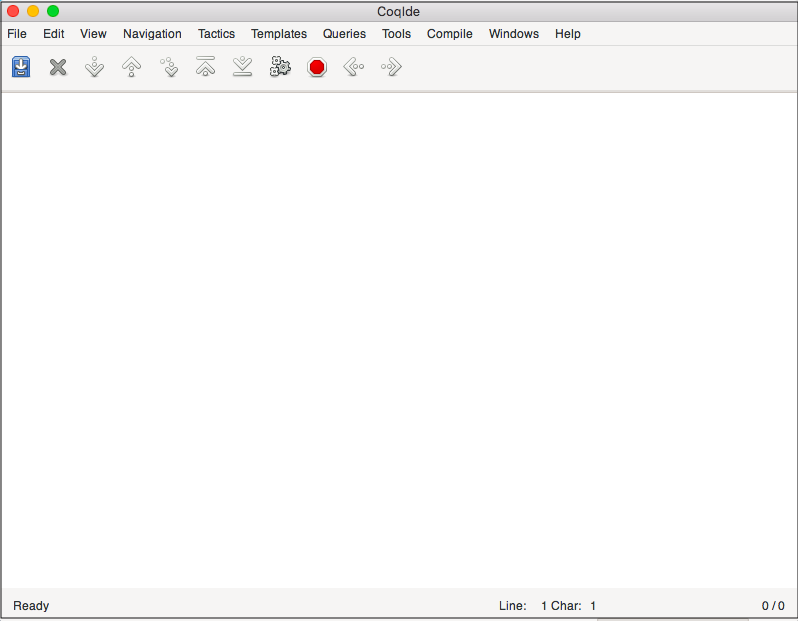
\includegraphics[width=\halfsize]
        		{CoqScreenshots/emptyIDE.png}
	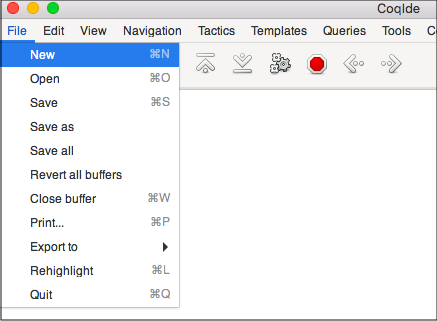
\includegraphics[width=\halfsize]
        		{CoqScreenshots/FixEmptyIDE.png}}
        
        \label{fig:IDEempty} 
        \captionof{figure}{CoqIDE v8.10.2  
        (a) empty IDE screen (b) getting new scratch script buffer open }
\end{minipage}

~\\
Go to "File" then "New" to get a new scratch script buffer open. 
















\newpage
\section{References}
	\label{Sec: refs}
	
Coq Proof Assistant Webpage 		\\
\url{https://coq.inria.fr}

~\\
Coq Documentation \\
\url{https://coq.inria.fr/distrib/current/refman/}

~\\
Christine Paulin-Mohring's course notes on Coq 	\\
\url{https://www.lri.fr/~paulin/LASER/course-notes.pdf}

~\\
DeepSpec Summer School COQ Intensive July 2017	\\
\url{https://deepspec.org/event/dsss17/coq\_intensive.html}

~\\
Software Foundations Books		\\
\url{https://softwarefoundations.cis.upenn.edu}

~\\
Induction in Coq		\\
\url{http://www.cs.cornell.edu/courses/cs3110/2018sp/l/22-coq-induction/notes.html}

~\\
CompCert: Verified C Compiler		\\
\url{http://compcert.inria.fr/motivations.html}

~\\
CertiCrypt: Computer-Aided Cryptographic Proofs in Coq		\\
\url{http://certicrypt.gforge.inria.fr}

~\\
OCaml Language
\\ \url{https://ocaml.org}
\\ \url{https://en.wikipedia.org/wiki/OCaml}

~\\
SML Language
\\ \url{https://en.wikipedia.org/wiki/Standard_ML}
\\ \url{http://sml-family.org}
\\ \url{https://www.smlnj.org}


















\end{document}

